\documentclass[conference]{IEEEtran}

\usepackage[utf8]{inputenc}
\usepackage[T1]{fontenc}
\usepackage[brazilian]{babel}
\usepackage{amsmath,amssymb,amsfonts}
\usepackage{graphicx}
\usepackage{booktabs}
\usepackage{array}
\usepackage{cite}
\usepackage{float}
\usepackage{algorithm}
\usepackage{algpseudocode}
\usepackage[hidelinks]{hyperref}

\floatname{algorithm}{Algoritmo}
\algrenewcommand\algorithmicrequire{\textbf{Entrada:}}
\algrenewcommand\algorithmicensure{\textbf{Saída:}}
\algrenewcommand\algorithmicif{\textbf{se}}
\algrenewcommand\algorithmicthen{\textbf{então}}
\algrenewcommand\algorithmicelse{\textbf{senão}}
\algrenewcommand\algorithmicfor{\textbf{para}}
\algrenewcommand\algorithmicwhile{\textbf{enquanto}}
\algrenewcommand\algorithmicdo{\textbf{faça}}
\algrenewcommand\algorithmicend{\textbf{fim}}
\algrenewcommand\algorithmicreturn{\textbf{retorne}}

\graphicspath{{figuras/}}

% Valores que dependem dos experimentos (critério de parada e execuções finais).
\newcommand{\Cparada}{300}

% Permite até 3 figuras/tabelas de largura dupla no topo de uma mesma página
% (o padrão é 1, o que empurra as figuras largas para o fim do documento).
\setcounter{dbltopnumber}{3}
\renewcommand{\dbltopfraction}{0.9}
\renewcommand{\dblfloatpagefraction}{0.8}

\begin{document}
\title{Otimização do Custo e \\Qualidade de Pilhas de Minério}

\author{
\IEEEauthorblockN{Saulo Bruno do Amaral - 2024425199}
\IEEEauthorblockN{Letícia Braga Esteves - 2023422609}
\IEEEauthorblockN{Yuri Wada Hirono Imokuti - 2023431004}
\IEEEauthorblockN{Roberto Júnior Cassimiro Campolina- 2023060480}
\IEEEauthorblockN{Juliana Goulart de Oliveira Duarte - 2024421690}
\IEEEauthorblockN{Igor Grieder Melo- 2025421316}\IEEEauthorblockA{
Universidade Federal de Minas Gerais -- UFMG\\
Belo Horizonte, Brasil
}
}

\maketitle

\section{Introdução}

O problema, proposto no case da disciplina~\cite{case_cassotis}, consiste na composição de pilhas de minério destinadas a dois equipamentos de sinterização. Cada pilha deve atingir uma massa final definida, respeitar limites de qualidade e utilizar apenas minérios compatíveis com o equipamento ao qual está associada. A decisão é realizada em unidades discretas de caminhões, cada um com capacidade fixa de 2 kt.

Na primeira entrega, o problema é tratado de forma mono-objetivo. São consideradas separadamente três funções objetivo: minimização do custo total de aquisição dos minérios, minimização do desvio quadrático do teor de SiO$_2$ em relação ao valor-alvo e minimização do desvio quadrático do teor de Al$_2$O$_3$ em relação ao valor-alvo.

A solução computacional é construída a partir de uma representação discreta das pilhas: cada pilha é um vetor em que cada posição corresponde a um caminhão e armazena o minério que ele transporta. Sobre essa representação, aplica-se a metaheurística GVNS (\textit{General Variable Neighborhood Search})~\cite{aula02}, com três estruturas de vizinhança e busca local do tipo VND. A solução inicial é gerada por uma heurística construtiva e, caso viole os limites de qualidade, é corrigida por um procedimento de reparo antes do início da busca. Como o método é estocástico, cada objetivo é otimizado em cinco execuções com sementes distintas. Na segunda etapa, os três objetivos são considerados conjuntamente pelas abordagens Soma Ponderada e $\varepsilon$-restrito, reutilizando a mesma GVNS.

Na terceira etapa, as receitas não dominadas da união das duas abordagens são as alternativas de uma decisão multicritério com quatro critérios: os três objetivos e a homogeneidade da receita das pilhas de cada equipamento. O ELECTRE~I reduz o conjunto às alternativas que nenhuma outra supera, o AHP escolhe entre elas a solução final, e uma análise de sensibilidade mede o quanto essa escolha depende dos parâmetros adotados.

O restante do relatório está organizado da seguinte forma. A Seção~\ref{sec:formulacao} apresenta a formulação matemática do problema. As Seções~\ref{sec:representacao} e~\ref{sec:construtiva} descrevem a representação computacional da solução e a heurística construtiva. A Seção~\ref{sec:gvns} detalha a GVNS, incluindo as vizinhanças, a busca local, a perturbação e o tratamento de soluções inviáveis. A Seção~\ref{sec:planejamento} descreve o planejamento experimental, e a Seção~\ref{sec:resultados} apresenta e discute os resultados. A Seção~\ref{sec:multi} apresenta as duas abordagens multiobjetivo, e a Seção~\ref{sec:decisao}, a decisão multicritério e sua análise de sensibilidade. Por fim, a Seção~\ref{sec:conclusao} apresenta as conclusões.

\section{Formulação Matemática}\label{sec:formulacao}

\subsection{Conjuntos e Índices}

\begin{align}
I &= \{1,\ldots,|I|\}, \\
J &= \{1,\ldots,|J|\}, \\
S &= \{1,\ldots,|S|\}, \\
K &= \{1,2\}.
\end{align}

\begin{align}
k=1 &\rightarrow \mathrm{SiO_2}, \\
k=2 &\rightarrow \mathrm{Al_2O_3}.
\end{align}

\subsection{Parâmetros}

\begin{table}[htbp]
\caption{Parâmetros do problema}
\centering
\begin{tabular}{p{0.20\columnwidth} p{0.70\columnwidth}}
\toprule
\textbf{Símbolo} & \textbf{Parâmetro} \\
\midrule
$P_j$ & Preço do minério $j$ (R\$/t) \\
$F_{kj}$ & Teor da substância $k$ no minério $j$ \\
$D_j^{\min}$ & Disponibilidade mínima do minério $j$ \\
$D_j^{\max}$ & Disponibilidade máxima do minério $j$ \\
$M_i$ & Massa da pilha $i$ (kt) \\
$T$ & Capacidade de um caminhão (kt) \\
$B_{sj}$ & Compatibilidade entre o sinter $s$ e o minério $j$ \\
$L_{ks}^{\min}$ & Limite mínimo da substância $k$ no sinter $s$ \\
$L_{ks}^{\max}$ & Limite máximo da substância $k$ no sinter $s$ \\
$L_{ks}^{\mathrm{alvo}}$ & Valor-alvo da substância $k$ no sinter $s$ \\
$s(i)$ & Sinter associado à pilha $i$ \\
\bottomrule
\end{tabular}
\label{tab:parametros}
\end{table}

\subsection{Variáveis de Decisão}

Seja $x_{ij}$ a quantidade de caminhões contendo o minério $j$ destinados à pilha $i$.

\begin{equation}
 x_{ij} \in \mathbb{Z}_{\geq 0},
 \qquad \forall i\in I,\ \forall j\in J
\end{equation}

\subsection{Teor das Pilhas}

\begin{equation}
L_{ki}
=
\frac{T}{M_i}
\sum_{j\in J} x_{ij} F_{kj}
\end{equation}

\subsection{Funções Objetivo}

\subsubsection{Minimização do custo}

\begin{equation}
\min f_1(x)
=
1000\,T
\sum_{i\in I}
\sum_{j\in J}
P_j x_{ij}
\end{equation}

O fator 1000 converte a capacidade do caminhão de kt para t, compatível com o preço em R\$/t, de modo que $f_1$ é expresso em reais. Com $T = 2$~kt, cada caminhão do minério $j$ custa $2\,000\,P_j$ reais.

\subsubsection{Minimização do desvio de SiO$_2$}

\begin{equation}
\min f_2(x)
=
\sum_{i\in I}
\left(
L_{1i}
-
L_{1,s(i)}^{\mathrm{alvo}}
\right)^2
\end{equation}

\subsubsection{Minimização do desvio de Al$_2$O$_3$}

\begin{equation}
\min f_3(x)
=
\sum_{i\in I}
\left(
L_{2i}
-
L_{2,s(i)}^{\mathrm{alvo}}
\right)^2
\end{equation}

\subsection{Restrições}

\subsubsection{Massa das pilhas}

\begin{equation}
T
\sum_{j\in J}
x_{ij}
=
M_i,
\qquad \forall i\in I
\end{equation}

\subsubsection{Qualidade}

\begin{equation}
L_{k,s(i)}^{\min}
\leq
L_{ki}
\leq
L_{k,s(i)}^{\max},
\qquad
\forall i\in I,\ \forall k\in K
\end{equation}

\subsubsection{Compatibilidade}

\begin{equation}
x_{ij}
\leq
\frac{M_i}{T}
B_{s(i),j},
\qquad
\forall i\in I,\ \forall j\in J
\end{equation}

\subsubsection{Disponibilidade}

\begin{equation}
D_j^{\min}
\leq
\sum_{i\in I} x_{ij}
\leq
D_j^{\max},
\qquad
\forall j\in J
\end{equation}

\subsubsection{Domínio}

\begin{equation}
x_{ij} \in \mathbb{Z}_{\geq 0},
\qquad
\forall i\in I,\ \forall j\in J
\end{equation}

\section{Representação Computacional da Solução}\label{sec:representacao}

\subsection{Representação de uma Pilha}
A pilha $i$ é representada por um vetor $s_i$ de comprimento
$n_i=M_i/T$. Cada posição contém o identificador do minério de um caminhão.
Assim, a massa é preservada mantendo o comprimento do vetor. P1 contém dez
posições; P10 contém dezenove. A ordem dos caminhões não altera a receita,
os teores nem os objetivos.

\subsection{Representação da Solução Completa}
O plano $s=(s_1,\ldots,s_{10})$ reúne as dez pilhas e 145 caminhões.
Cada pilha tem seu equipamento de destino fixado nos dados. No Python,
os identificadores internos dos minérios são $0,\ldots,19$; nos dados,
nas tabelas e na formulação matemática são $1,\ldots,20$.

\subsection{Relação com $x_{ij}$}
Seja $s_{ir}$ o minério do caminhão na posição $r$ do vetor da pilha $i$.
A variável $x_{ij}$ da formulação é obtida contando quantas posições desse
vetor contêm o minério $j$:
\begin{equation}
x_{ij}=\bigl|\{\,r\in\{1,\ldots,n_i\} : s_{ir}=j\,\}\bigr|.
\end{equation}
Por exemplo, se o vetor de P1 for
$(\mathrm{M14},\mathrm{M14},\mathrm{M14},\mathrm{M14},\mathrm{M14},\mathrm{M14},\mathrm{M13},\mathrm{M4},\mathrm{M10},\mathrm{M11})$,
então $x_{1,14}=6$, $x_{1,13}=x_{1,4}=x_{1,10}=x_{1,11}=1$ e $x_{1,j}=0$
para os demais minérios.

A ordem das posições não altera $x_{ij}$: dois vetores com os mesmos minérios
em ordens diferentes descrevem a mesma pilha, com o mesmo custo e os mesmos
teores. Por isso, os resultados são exportados como matrizes de contagens
$x_{ij}$, e as vizinhanças não geram movimentos que diferem apenas pela
posição escolhida entre caminhões do mesmo minério, pois eles produziriam
o mesmo vizinho.

\subsection{Verificação de Viabilidade}
A rotina \texttt{evaluate} verifica comprimento, identificadores e
elegibilidade e calcula qualidade e uso global de cada minério. Um erro
estrutural interrompe a avaliação; violações de qualidade ou disponibilidade
formam a medida usada no reparo. Na GVNS mono-objetivo e na Soma Ponderada,
a admissibilidade exige violação física zero. No método $\varepsilon$-restrito,
exige adicionalmente o atendimento dos dois limites agregados definidos
na Seção~\ref{sec:multi}.

\subsection{Avaliação Incremental}
Todos os objetivos e restrições são somas de parcelas por pilha, mais o uso
global de cada minério. Cada vizinho copia apenas as pilhas que altera
(uma em $N_1$ e $N_3$, duas em $N_2$) e compartilha as demais com a solução
de origem. A avaliação reaproveita as parcelas das pilhas não alteradas e
recalcula só as alteradas, atualizando o uso dos minérios pela diferença.
A ordem das somas é a mesma da avaliação completa, de modo que os valores
são idênticos em ponto flutuante; um teste automatizado confere essa
igualdade. A mudança não altera a busca: com as mesmas sementes, as
trajetórias são idênticas às da avaliação completa, e o tempo por execução
caiu cerca de 2,7 vezes em um teste com $f_3$.

\section{Heurística Construtiva}\label{sec:construtiva}

\subsection{Geração da Solução Inicial}

A solução inicial segue a sugestão do enunciado e é gerada em duas etapas determinísticas: primeiro, são distribuídos os caminhões dos minérios com disponibilidade mínima obrigatória; depois, as posições restantes de cada pilha são preenchidas com os minérios elegíveis mais baratos. Por construção, a solução respeita a massa das pilhas, a compatibilidade entre minérios e sinters e os limites de disponibilidade; apenas os limites de qualidade podem ser violados.

Em ambas as etapas, antes de confirmar cada caminhão, verifica-se se ainda é possível completar todas as pilhas: a capacidade restante de cada sinter não pode exceder a disponibilidade máxima ainda livre dos minérios elegíveis para ele. Se a escolha tornaria o preenchimento impossível, ela é desfeita e o próximo candidato é testado.

\subsection{Atendimento das Disponibilidades Mínimas}

Na instância utilizada, quatro minérios têm uso mínimo obrigatório: M4 (2 caminhões), M10 (2), M11 (1) e M20 (1). Os minérios exclusivos de um sinter (M10, M11 e M20) são distribuídos primeiro, pois têm menos pilhas possíveis; em seguida, é distribuído o M4, que é elegível para os dois sinters. Os caminhões de cada minério são alocados em rodízio entre as pilhas elegíveis, de modo que o uso mínimo não se concentre em uma única pilha.

\subsection{Preenchimento das Pilhas}

As pilhas são completadas em ordem, de P1 a P10. Para cada posição livre, escolhe-se o minério mais barato que seja elegível para o sinter da pilha e que ainda não tenha atingido sua disponibilidade máxima. Essa regra gera uma solução de baixo custo, mas que tende a violar os limites de qualidade, já que vários dos minérios mais baratos da instância, como M13, M15 e M17, têm teores elevados de SiO$_2$ e Al$_2$O$_3$.

\subsection{Tratamento de Inviabilidade Inicial}

Se a solução construída violar algum limite de qualidade, um procedimento de reparo busca uma primeira solução viável antes do início da GVNS. O reparo tem a mesma estrutura da GVNS (perturbação seguida de VND), mas, em vez do objetivo, minimiza a violação total
\begin{align}
v_{ki} &= \max\{0,\, L_{k,s(i)}^{\min} - L_{ki}\} \nonumber \\
       &\quad + \max\{0,\, L_{ki} - L_{k,s(i)}^{\max}\}, \\
V(x)   &= \sum_{i \in I} \sum_{k \in K}
          \frac{v_{ki}}{L_{k,s(i)}^{\max} - L_{k,s(i)}^{\min}} + V_D(x),
\end{align}
em que $v_{ki}$ é o quanto o teor da substância $k$ na pilha $i$ está fora dos limites do seu sinter e $V_D(x)$ é a violação dos limites de disponibilidade, calculada de forma análoga. Cada violação é dividida pela amplitude do intervalo permitido, para que substâncias e minérios com escalas diferentes contribuam de forma comparável. O reparo termina assim que qualquer solução admissível é avaliada. Cada ciclo de reparo (perturbação seguida de VND) consome um ciclo do mesmo orçamento $C$ da GVNS, descrito na Seção~\ref{sec:gvns}. Se o reparo completar $R=100$ ciclos sem encontrar solução admissível, ele recomeça a partir da construção. Como o gerador pseudoaleatório já avançou, a nova tentativa percorre outra sequência de perturbações e vizinhos. Esse reinício se repete até que uma solução admissível seja encontrada ou até que o orçamento de $C$ ciclos se esgote. No segundo caso, a execução é registrada como falha de reparo, sem solução exportada, e o lote prossegue com a execução seguinte; a falha não prova que a configuração seja inviável. Cada execução registra quantos ciclos de reparo e quantos reinícios utilizou. A fase de otimização só começa após o reparo e usa os ciclos restantes do orçamento. A violação $V$ é usada apenas no reparo e nunca é somada aos objetivos.

Com esse reinício, uma falha do reparo nunca interrompe o lote de execuções. Em todas as execuções mono-objetivo realizadas, o reparo encontrou uma solução viável no primeiro ciclo.

\section{Metaheurística GVNS}\label{sec:gvns}

\subsection{Estrutura Geral}

Foi adotada a GVNS (\textit{General Variable Neighborhood Search})~\cite{aula02}, variante da VNS em que a busca local é, ela própria, uma descida em vizinhanças variáveis (VND). A cada ciclo, a solução corrente é perturbada em uma vizinhança $N_k$, a perturbação é refinada pela VND, que percorre $N_1$, $N_2$ e $N_3$, e o resultado é aceito ou não. As três vizinhanças atuam diretamente sobre a composição das pilhas, como pede o enunciado, e são descritas a seguir. A GVNS é executada separadamente para cada objetivo, sempre com as mesmas restrições.

\subsection{Vizinhança $N_1$}

A vizinhança $N_1$ corresponde à sugerida no enunciado: escolhe-se uma pilha e uma posição do seu vetor e troca-se o minério dessa posição por outro minério elegível para o sinter da pilha. O movimento altera um único caminhão, preserva a massa e a compatibilidade, e pode violar a qualidade da pilha ou a disponibilidade do minério.

Como a composição, os objetivos e as restrições dependem apenas de quantos caminhões de cada minério há na pilha, e não da ordem das posições, posições com o mesmo minério na mesma pilha são equivalentes. Por isso, cada par (minério atual, minério novo) de uma pilha é gerado uma única vez, o que evita avaliar vizinhos repetidos.

\subsection{Vizinhança $N_2$}

A vizinhança $N_2$ também segue o enunciado: escolhem-se duas pilhas $p_1$ e $p_2$ e um minério de cada uma; se o minério de $p_1$ for elegível para o sinter de $p_2$ e vice-versa, os dois caminhões são trocados. O movimento preserva a massa das pilhas e o uso total de cada minério, portanto nunca viola a disponibilidade; pode, porém, violar a qualidade de uma das duas pilhas. Assim como em $N_1$, trocas entre posições equivalentes são geradas uma única vez. A ordem de exploração sorteia diretamente os pares de pilhas, e não apenas as pilhas, para que todo par tenha a mesma chance de ser examinado primeiro; percorrer os pares a partir de uma única pilha sorteada esgotaria os pares dessa pilha antes dos demais e concentraria a perturbação e a primeira melhora nela.

\subsection{Vizinhança $N_3$}

A vizinhança $N_3$ foi definida neste trabalho. Ela mantém nove pilhas fixas e reconstrói a composição inteira da décima, exigindo que pelo menos $m_i$ dos seus $n_i$ caminhões mudem de minério, sendo
\begin{equation}
m_i=\max\{2,\ \lceil \phi\, n_i\rceil\}
\label{eq:n3min}
\end{equation}
com $\phi=0{,}25$. Assim, uma pilha de 10 caminhões muda ao menos 3 caminhões, e uma de 19 caminhões, ao menos 5. O piso de dois caminhões garante que $N_3$ nunca gere um movimento da vizinhança de $N_1$.

A nova composição é gerada diretamente como contagens de caminhões por minério, e não como permutações de posições. Durante a enumeração, o número de caminhões de cada minério é limitado pela disponibilidade que resta após o uso nas outras nove pilhas, e combinações que não podem atingir os limites de qualidade da pilha são descartadas antecipadamente. Assim, a pilha reconstruída sempre respeita massa, compatibilidade, disponibilidade e qualidade; se as outras nove pilhas já forem viáveis, o vizinho inteiro é viável. Durante a GVNS, em que a solução corrente é sempre viável, $N_3$ funciona, portanto, como um operador que preserva a viabilidade.

As vizinhanças são complementares: $N_1$ ajusta uma receita, $N_2$ redistribui minérios entre pilhas sem alterar seu uso total, e $N_3$ avalia uma mudança maior e coordenada. A reconstrução permite avaliar diretamente a nova receita, sem exigir que cada alteração intermediária seja viável ou melhore o objetivo; isso pode contornar bloqueios dos movimentos pequenos. Não se afirma que a mesma receita só possa ser alcançada por $N_3$. A exigência de mudar uma fração mínima dos caminhões distingue esse movimento de uma substituição isolada ou de uma troca entre pilhas, e faz de $N_3$ a vizinhança de maior alteração, coerente com a ordem $N_1$, $N_2$, $N_3$ da VND e da perturbação.

Uma fração maior, como metade da pilha, excluiria todos os movimentos intermediários, entre dois caminhões e metade da pilha, que nenhuma das outras vizinhanças cobre. O valor $\phi=0{,}25$ foi escolhido por um experimento com oito regras, descrito na Seção~\ref{sec:resultados}. O experimento mostrou também que, para $\phi\geq0{,}4$, a vizinhança fica praticamente vazia perto de boas soluções de $f_2$ e $f_3$: com as outras nove pilhas fixas e os limites de disponibilidade, quase não existe receita que respeite a qualidade e altere tantos caminhões. Com uma fração alta, portanto, $N_3$ deixaria de contribuir para esses dois objetivos depois do início da busca.

$N_3$ não possui teto de candidatos completos, nós de enumeração ou tempo. A VND percorre seus vizinhos em ordem sorteada até a primeira melhora ou o esgotamento das reconstruções possíveis. A enumeração é finita, pois trabalha com contagens inteiras limitadas pela massa e pelas disponibilidades. Para que a enumeração completa seja viável, a VND descarta, além dos ramos que não atingem os limites de qualidade, os ramos que não podem melhorar o critério ativo. Como as outras nove pilhas ficam fixas e cada objetivo é uma soma de parcelas por pilha, a variação do critério é a variação ponderada das parcelas da pilha reconstruída. Em cada ramo parcial, calcula-se um limitante inferior para essa variação: o custo mínimo de completar a pilha com os caminhões restantes e o menor desvio quadrático possível dentro da faixa de teor ainda alcançável. Se o limitante indica que nenhuma receita do ramo melhora o critério, o ramo é descartado. Esse corte não altera a vizinhança nem a regra de primeira melhora, pois só elimina receitas que a VND rejeitaria. Na perturbação e no reparo, os cortes por critério não são aplicados.

Um teto no número de receitas examinadas por visita limitaria as receitas avaliadas, mas não o esforço de enumeração: antes de cada receita completa, podem ser visitadas muitas combinações parciais. Com os cortes, nenhum teto é necessário, e a vizinhança é examinada por completo. O esforço da enumeração é registrado à parte, como número de nós visitados, pois esses cálculos não entram no contador de avaliações de soluções completas.

\subsection{Busca Local}

A busca local é uma VND (\textit{Variable Neighborhood Descent}) com estratégia de primeira melhora (Algoritmo~\ref{alg:vnd}). As vizinhanças são exploradas na ordem $N_1$, $N_2$, $N_3$, da menor para a maior alteração. Os vizinhos de cada vizinhança são percorridos em ordem aleatória, e o primeiro que melhora o critério é aceito; a busca, então, volta para $N_1$. Se nenhum vizinho de $N_\ell$ melhora, passa-se para $N_{\ell+1}$. No modo de otimização, a busca termina quando as três vizinhanças são esgotadas sem melhora, produzindo um ótimo local em $N_1$, $N_2$ e $N_3$, segundo os operadores implementados e a tolerância numérica. No reparo, retorna assim que encontra uma solução viável. Nenhuma dessas condições prova ótimo global.

A primeira melhora foi preferida à melhor melhora porque $N_2$ e $N_3$ têm muitos vizinhos, e examinar todos a cada passo tornaria cada ciclo muito mais caro. A ordem aleatória dos vizinhos faz com que execuções com sementes diferentes explorem regiões diferentes do espaço de busca.

\subsection{Perturbação}

A perturbação (\textit{shaking}) tenta até $k$ movimentos sucessivos da vizinhança $N_k$, com $k \in \{1,2,3\}$. Em cada tentativa, escolhe o primeiro vizinho viável na ordem sorteada, mesmo que piore o objetivo. Se nenhum existir, a solução permanece igual naquela tentativa. Assim, tenta uma substituição em $N_1$, até duas trocas em $N_2$ ou até três reconstruções em $N_3$; uma mesma pilha pode ser reconstruída mais de uma vez. A intensidade cresce, portanto, tanto pela vizinhança quanto pelo número de movimentos, o que produz perturbações progressivamente mais fortes quando a busca não encontra melhora. Depois das tentativas, aplica uma VND. Seu resultado é comparado com a solução anterior à perturbação: se melhorar, é aceito e $k$ volta a 1; caso contrário, a solução anterior é mantida e $k$ avança circularmente.

\subsection{Tratamento de Soluções Inviáveis}

O enunciado admite várias políticas para os movimentos que violam restrições. Para este trabalho, foi adotada uma combinação de três delas:
\begin{itemize}
    \item \textbf{reparo} da solução construtiva, quando ela é inviável, antes do início da GVNS;
    \item \textbf{rejeição} dos movimentos inviáveis durante a GVNS: todos os candidatos são verificados segundo as restrições ativas antes de serem usados na busca local ou na perturbação;
    \item \textbf{operador que preserva a viabilidade física}, no caso de $N_3$, quando parte de um plano fisicamente viável. No reparo, as pilhas fixas podem continuar inviáveis; no método $\varepsilon$-restrito, os limites agregados também precisam ser verificados.
\end{itemize}

A alternativa de aceitar soluções inviáveis com penalização~\cite{aula04} foi descartada porque exigiria calibrar pesos de penalidade para cada objetivo, cujas escalas são muito diferentes (milhões de reais em $f_1$ e unidades de pp$^2$ em $f_2$ e $f_3$). Com a rejeição, a GVNS trabalha sempre sobre soluções viáveis, e o valor registrado de $f$ é sempre o de uma solução que atende a todas as restrições. Essa política impede aceitar passos intermediários inviáveis. A reconstrução coordenada de $N_3$ pode contornar alguns desses bloqueios, sem garantir acesso a toda região viável.

\subsection{Critério de Aceitação}

Após a VND, a nova solução substitui a solução corrente somente se tiver valor do objetivo estritamente menor; nesse caso, $k$ volta a 1. Caso contrário, a solução corrente é mantida e $k$ avança. Independentemente da aceitação, a melhor solução viável avaliada ao longo de toda a execução, incluindo as avaliadas no reparo, na perturbação e na busca local, é armazenada e é a solução retornada. Em todas as comparações (viabilidade, melhora na VND, aceitação e registro da melhor solução), diferenças de até $10^{-10}$ são tratadas como erro de arredondamento, com a mesma tolerância em todos os pontos do algoritmo.

\subsection{Critério de Parada}

Cada execução dispõe de um orçamento de $C=\Cparada$ ciclos, somando os ciclos de reparo e os ciclos globais da GVNS, cada um composto por perturbação e VND. Não é um limite por vizinhança nem um número de avaliações; o tempo de cada ciclo depende da enumeração e das melhorias encontradas. Nenhum limite de tempo interrompe a busca.

Com 50 ciclos, a busca é interrompida antes da convergência: execuções com 200 ciclos e as mesmas sementes melhoraram o resultado de 50 ciclos em todos os objetivos. O valor de $C$ foi escolhido a partir de execuções longas, descritas na Seção~\ref{sec:resultados}.

\subsection{Pseudocódigo}

O Algoritmo~\ref{alg:gvns} apresenta a metaheurística completa, e o Algoritmo~\ref{alg:vnd}, a busca local VND usada tanto no reparo quanto na GVNS. Nos dois, $f$ é o critério escalar ativo: um dos objetivos isolados, a Soma Ponderada ou o custo normalizado no método $\varepsilon$-restrito. $V(x)$ é a medida de violação ativa: física nas versões mono-objetivo e Soma Ponderada, ou $V_\varepsilon$ na versão $\varepsilon$-restrito. Com as tolerâncias numéricas, $V(x)=0$ caracteriza uma solução admissível para a chamada. As definições multiobjetivo estão na Seção~\ref{sec:multi}. Em qualquer ponto do algoritmo, toda solução viável avaliada que melhora $f$ passa a ser a melhor solução $x^*$.

\begin{algorithm}[!t]
\caption{Metaheurística GVNS}
\label{alg:gvns}
\begin{algorithmic}[1]
\Require critério $f$, violação ativa $V$, ciclos $C$, reinício $R$, semente
\Ensure melhor solução viável $x^*$, ou falha de reparo
\State $x \gets \Call{Construir}{\,}$
\Comment{mínimos + menor preço}
\State $c \gets 0$
\If{$V(x) = 0$}
    \State $x^* \gets x$
\Else
    \State $k \gets 1$
    \Comment{reparo}
    \While{não há $x^*$ \textbf{e} $c < C$}
        \If{$R$ ciclos de reparo desde o último início}
            \State $x \gets \Call{Construir}{\,}$;\ $k \gets 1$
            \Comment{reinício}
        \EndIf
        \State $c \gets c + 1$
        \State $x' \gets$ perturbar $x$ em $N_k$, até $k$ movimentos existentes
        \State avaliar $x'$ e atualizar $x^*$ se viável
        \If{há $x^*$} \State \textbf{interrompe o laço} \EndIf
        \State $x' \gets \Call{VND}{x', V, \text{reparo}}$
        \If{$V(x') < V(x)$}
            \State $x \gets x'$;\ $k \gets 1$
        \Else
            \State $k \gets (k \bmod 3) + 1$
        \EndIf
    \EndWhile
\EndIf
\If{não há $x^*$} \State \Return falha de reparo \EndIf
\State $x \gets x^*$;\ $k \gets 1$
\Comment{GVNS}
\For{$c \gets c+1$ \textbf{até} $C$}
    \State $x' \gets x$
    \Comment{perturbação}
    \For{até $k$ tentativas}
        \State $y \gets$ 1º vizinho viável de $x'$ em $N_k$, se existir
        \If{$y$ existe} \State $x' \gets y$ \EndIf
    \EndFor
    \State $x'' \gets \Call{VND}{x', f, \text{otimização}}$
    \If{$f(x'') < f(x)$}
    \Comment{aceitação}
        \State $x \gets x''$;\ $k \gets 1$
    \Else
        \State $k \gets (k \bmod 3) + 1$
    \EndIf
\EndFor
\State \Return $x^*$
\end{algorithmic}
\end{algorithm}

\begin{algorithm}[!t]
\caption{Busca local VND}
\label{alg:vnd}
\begin{algorithmic}[1]
\Require solução $x$, critério $g$ ($V$ ou $f$), modo
\Ensure solução refinada; na otimização, ótimo local em $N_1$, $N_2$, $N_3$
\State $\ell \gets 1$
\While{$\ell \le 3$}
    \State $melhorou \gets$ falso
    \For{cada $y \in N_\ell(x)$, em ordem aleatória}
        \If{modo = reparo \textbf{e} $V(y) = 0$}
            \State \Return $y$
        \EndIf
        \If{modo = otimização \textbf{e} $V(y) > 0$}
            \State \textbf{continue} para o próximo vizinho
            \Comment{rejeita inviável}
        \EndIf
        \If{$g(y) < g(x)$}
        \Comment{primeira melhora}
            \State $x \gets y$;\ $\ell \gets 1$;\ $melhorou \gets$ verdadeiro
            \State \textbf{interrompe o laço}
        \EndIf
    \EndFor
    \If{\textbf{não} $melhorou$} \State $\ell \gets \ell + 1$ \EndIf
\EndWhile
\State \Return $x$
\end{algorithmic}
\end{algorithm}

\section{Planejamento Experimental}\label{sec:planejamento}

\subsection{Configuração dos Experimentos}

Os experimentos utilizam a instância de exemplo do anexo do case, com 20 minérios, 10 pilhas (P1--P5 no Sinter~1 e P6--P10 no Sinter~2) e caminhões de 2~kt. O algoritmo foi implementado em Python~3.14, sem bibliotecas de otimização; o Matplotlib é usado apenas para gerar as figuras e o SciPy apenas para os testes estatísticos e, na decisão multicritério, para as componentes fortemente conexas do grafo do ELECTRE~I; o NumPy calcula os autovetores do AHP. Cada um dos três objetivos é otimizado separadamente, sempre com o mesmo conjunto de restrições.

\subsection{Parâmetros do Algoritmo}

A Tabela~\ref{tab:parametros_alg} resume os parâmetros da implementação. Nenhum deles é fixado pelo enunciado.

\begin{table}[htbp]
\caption{Parâmetros do algoritmo}
\centering
\begin{tabular}{p{0.55\columnwidth} r}
\toprule
\textbf{Parâmetro} & \textbf{Valor} \\
\midrule
Orçamento de ciclos por execução, $C$ (reparo + GVNS) & \Cparada \\
Fração mínima alterada por $N_3$, $\phi$ & 0{,}25 \\
Ciclos de reparo antes de reiniciar, $R$ & 100 \\
Teto de candidatos de $N_3$ & Sem teto \\
Tolerância numérica das comparações & $10^{-10}$ \\
Semente base & 2026 \\
\bottomrule
\end{tabular}
\label{tab:parametros_alg}
\end{table}

Os valores de $\phi$ e de $C$ foram escolhidos por experimentos próprios, apresentados na Seção~\ref{sec:resultados}. O valor de $R$ não foi calibrado, pois o reparo encontrou solução viável no primeiro ciclo em todas as execuções realizadas; ele apenas define quando uma tentativa de reparo sem sucesso é abandonada. O esforço completo de uma visita a $N_3$ pode incluir muitas combinações parciais antes de gerar uma receita. Por isso, além das avaliações, registra-se o número de nós visitados na enumeração.

Os tempos medidos refletem a concorrência entre processos executados em paralelo e não estimam precisamente a duração de uma execução sequencial.

\subsection{Referência Exata}
Para medir a distância entre a GVNS e o ótimo global, os três problemas mono-objetivo também foram resolvidos pelo solver Gurobi~13 com a formulação da Seção~\ref{sec:formulacao}: $f_1$ como programa linear inteiro e $f_2$ e $f_3$ como programas quadráticos inteiros convexos. Esses valores servem apenas de comparação; não são usados na GVNS, na normalização nem em nenhuma outra etapa do trabalho.

\subsection{Número de Execuções}

Como a GVNS é estocástica, cada objetivo foi otimizado em cinco execuções independentes, conforme exigido pelo enunciado, totalizando 15 execuções. Cada uma usa sua própria sequência pseudoaleatória; sementes diferentes não provam independência estatística perfeita. As execuções diferem apenas na semente do gerador de números aleatórios, que determina as escolhas feitas na perturbação e a ordem de exploração das vizinhanças. A semente da execução $r \in \{1,\ldots,5\}$ do objetivo $f_k$ é
\begin{equation}
\text{semente} = 2026 + 10\,000\,(k-1) + r,
\end{equation}
o que garante sementes distintas para as 15 execuções e torna todos os resultados reproduzíveis. A semente base foi fixada antes da realização dos experimentos e não foi escolhida com base nos resultados.

\subsection{Métricas Utilizadas}

Para cada objetivo, são registrados o valor da melhor solução viável de cada execução e, a partir dos cinco valores, o mínimo, a média, o desvio padrão amostral e o máximo. O esforço computacional é medido pelo número de avaliações de soluções candidatas, isto é, pelo número de vezes em que os objetivos e as restrições de uma solução são calculados, incluindo as avaliações feitas no reparo, na perturbação e na busca local. O tempo de execução também é registrado, mas apenas como informação complementar, pois depende da máquina e da carga do sistema.

\subsection{Critério de Comparação}

As execuções e as configurações do algoritmo são comparadas pelo valor final do objetivo otimizado. O mínimo indica a melhor solução encontrada; a média e o desvio padrão indicam a qualidade típica e a sensibilidade do método à semente. Também são registrados o número de avaliações, o número de nós da enumeração de $N_3$ e o tempo medido. As avaliações são uma contagem independente da máquina, mas não incluem os cálculos internos da enumeração de $N_3$, contados à parte.

Na escolha de parâmetros, as alternativas são comparadas com as mesmas sementes, execução a execução. Usa-se o teste de Friedman~\cite{friedman1937} para verificar se há diferença entre todas as alternativas e o teste de postos sinalizados de Wilcoxon~\cite{wilcoxon1945} para comparar pares; ambos são não paramétricos e pareados, adequados a amostras pequenas sem suposição de normalidade. O uso desses testes na comparação de metaheurísticas, com as condições de aplicação de cada um, é descrito por Derrac \textit{et al.}~\cite{derrac2011}. Os testes foram calculados com as funções \texttt{friedmanchisquare} e \texttt{wilcoxon} do SciPy~\cite{scipy2020}.

\subsection{Código-fonte e reprodutibilidade}

O código-fonte, os dados de entrada e as instruções para executar os experimentos estão disponíveis no repositório do projeto: \url{https://github.com/jlzht/td-tp}.

\section{Resultados e Discussões}\label{sec:resultados}

% Figuras de largura dupla só aparecem a partir da página seguinte à sua
% definição; por isso são definidas aqui, no início da seção de resultados.
\begin{figure*}[!t]
\centering
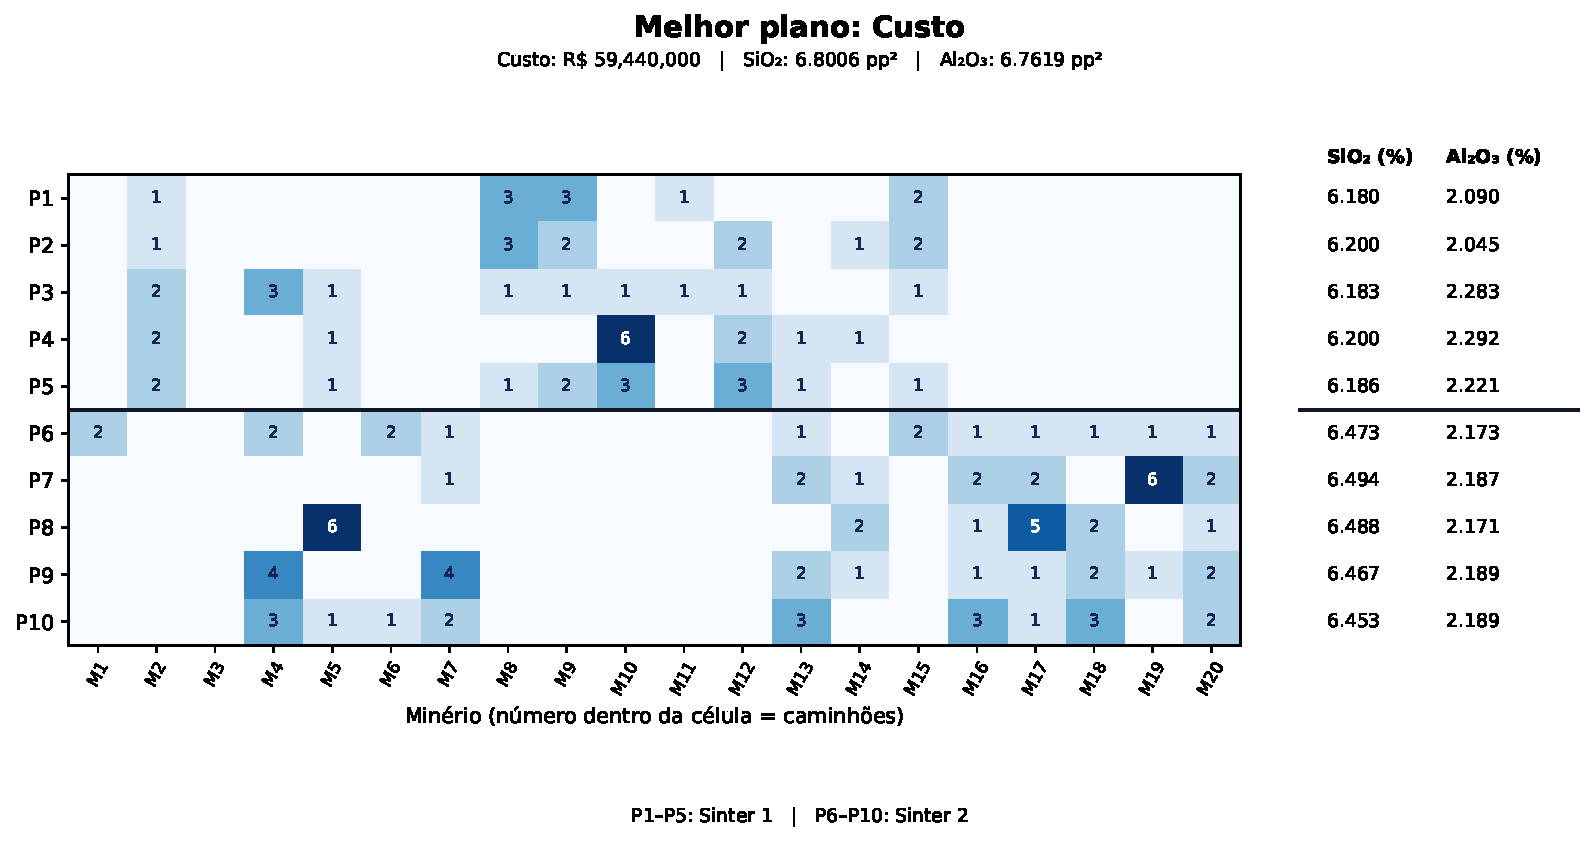
\includegraphics[width=0.85\textwidth]{melhor_f1.pdf}
\caption{Melhor solução encontrada para $f_1$ (execução 5).}
\label{fig:melhor_f1}
\end{figure*}

\begin{figure*}[!t]
\centering
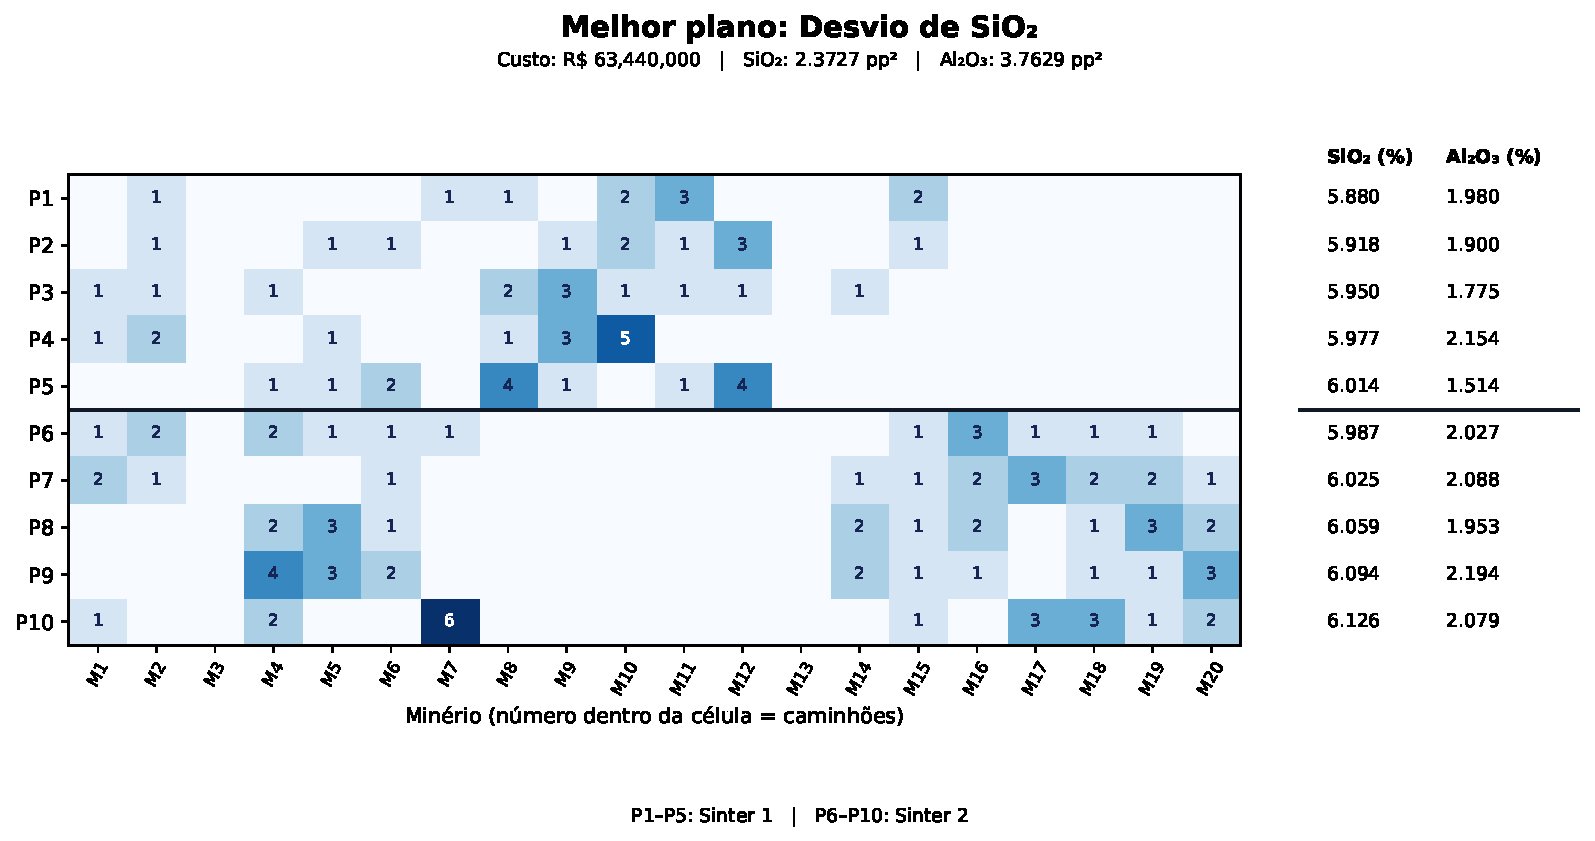
\includegraphics[width=0.85\textwidth]{melhor_f2.pdf}
\caption{Melhor solução encontrada para $f_2$ (execução 1).}
\label{fig:melhor_f2}
\end{figure*}

\begin{figure*}[!t]
\centering
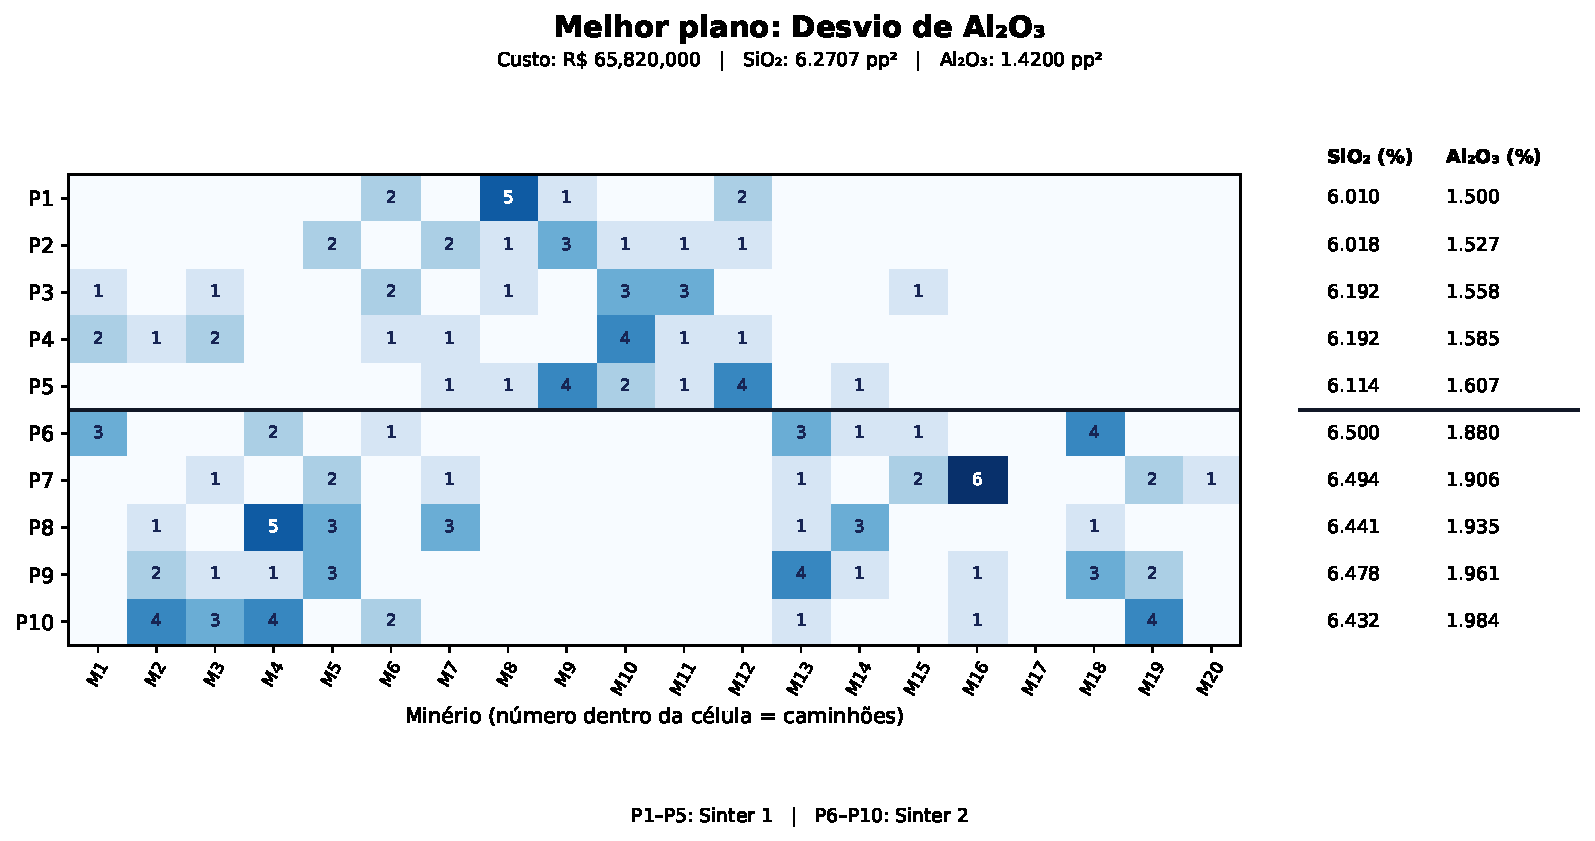
\includegraphics[width=0.85\textwidth]{melhor_f3.pdf}
\caption{Melhor solução encontrada para $f_3$ (execução 4).}
\label{fig:melhor_f3}
\end{figure*}

\begin{figure*}[!t]
\centering
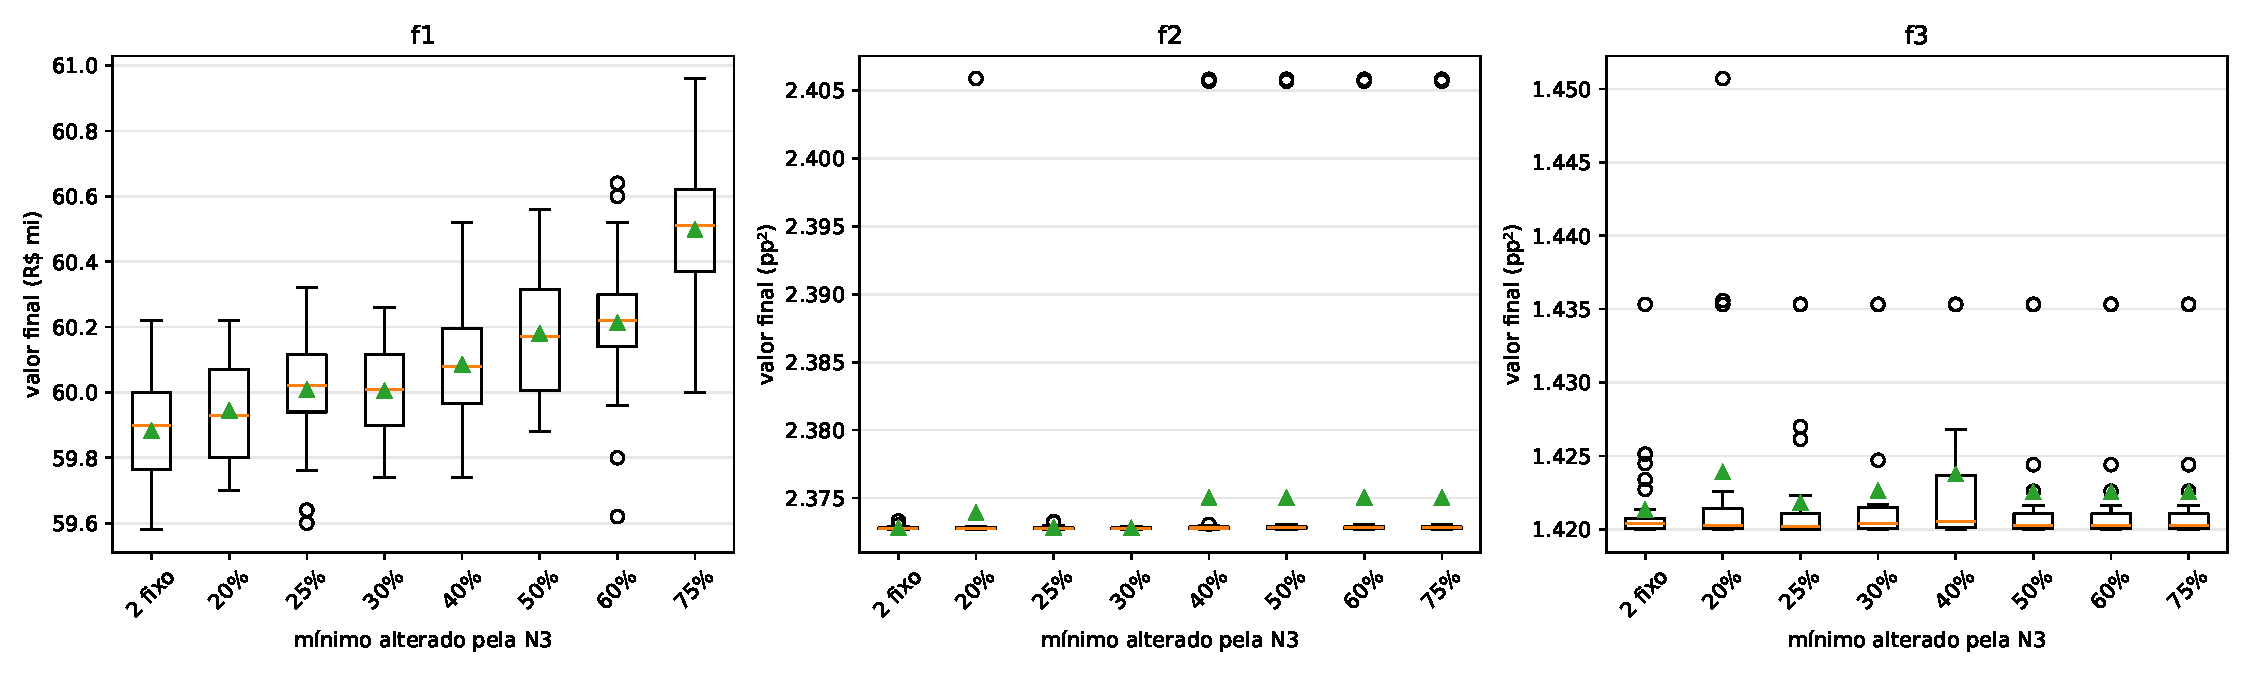
\includegraphics[width=\textwidth]{n3_fracoes.pdf}
\caption{Valor final de 30 execuções (50 ciclos) de cada objetivo para cada regra de mínimo alterado por $N_3$. Caixas: quartis; traço: mediana; triângulo: média; círculos: outliers.}
\label{fig:n3_fracoes}
\end{figure*}

\subsection{Escolha da Fração Mínima de $N_3$}\label{sec:escolha_phi}

Para escolher $\phi$, a GVNS foi executada com oito regras: mínimo fixo de dois caminhões ($\phi=0$) e $\phi\in\{0{,}20;0{,}25;0{,}30;0{,}40;0{,}50;0{,}60;0{,}75\}$, sempre com o arredondamento para cima da Equação~(\ref{eq:n3min}). Para cada regra e cada objetivo, foram feitas 30 execuções de 50 ciclos com as mesmas sementes, totalizando 720 execuções. Nesse experimento, $N_2$ explorava os pares a partir de uma pilha sorteada; essa condição é a mesma para todas as regras comparadas. A Tabela~\ref{tab:n3_fracoes} resume as médias e a Figura~\ref{fig:n3_fracoes} mostra a distribuição dos valores finais.

\begin{table}[htbp]
\caption{Média do valor final em 30 execuções por regra de $N_3$}
\centering
\begin{tabular}{l r r r}
\toprule
\textbf{Regra} & \textbf{$f_1$ (R\$ mi)} & \textbf{$f_2$ (pp$^2$)} & \textbf{$f_3$ (pp$^2$)} \\
\midrule
2 caminhões & \textbf{59{,}88} & 2{,}37280 & \textbf{1{,}42131} \\
$\phi=0{,}20$ & 59{,}94 & 2{,}37388 & 1{,}42387 \\
$\phi=0{,}25$ & 60{,}01 & 2{,}37281 & 1{,}42179 \\
$\phi=0{,}30$ & 60{,}00 & \textbf{2{,}37278} & 1{,}42261 \\
$\phi=0{,}40$ & 60{,}08 & 2{,}37499 & 1{,}42372 \\
$\phi=0{,}50$ & 60{,}18 & 2{,}37501 & 1{,}42251 \\
$\phi=0{,}60$ & 60{,}21 & 2{,}37501 & 1{,}42251 \\
$\phi=0{,}75$ & 60{,}50 & 2{,}37501 & 1{,}42251 \\
\bottomrule
\end{tabular}
\label{tab:n3_fracoes}
\end{table}

Em $f_1$, o teste de Friedman~\cite{friedman1937} indica diferença entre as regras ($p=2{,}6\times10^{-21}$), e o custo médio cresce com $\phi$. Na comparação pareada, $\phi=0{,}25$ foi melhor que $\phi=0{,}50$ em 23 das 30 execuções (Wilcoxon, $p=5{,}3\times10^{-5}$). Em $f_2$ ($p=0{,}16$) e $f_3$ ($p=0{,}76$), o teste de Friedman não indica diferença; as médias mais altas de algumas regras se devem a poucas execuções que terminaram em um mesmo valor ruim, visíveis como pontos isolados na Figura~\ref{fig:n3_fracoes}.

Em $f_2$ e $f_3$, as regras $\phi=0{,}50$, $0{,}60$ e $0{,}75$ produziram resultados idênticos em todas as 30 execuções, inclusive no número de avaliações. A causa foi verificada contando os vizinhos de $N_3$ a partir de uma solução obtida após três ciclos (Tabela~\ref{tab:n3_vazia}): nesses objetivos, a vizinhança fica vazia para $\phi\geq0{,}5$. Como a enumeração percorre os mesmos ramos e só rejeita as receitas completas que mudam poucos caminhões, a busca consome os mesmos sorteios e segue a mesma trajetória, sem que $N_3$ contribua. Com $\phi\geq0{,}5$, portanto, a busca de $f_2$ e $f_3$ dependeria apenas de $N_1$ e $N_2$ depois do início.

\begin{table}[htbp]
\caption{Vizinhos de $N_3$ a partir de uma solução após três ciclos}
\centering
\begin{tabular}{l r r r}
\toprule
\textbf{Regra} & \textbf{$f_1$} & \textbf{$f_2$} & \textbf{$f_3$} \\
\midrule
2 caminhões & 183\,642 & 2\,197 & 1\,684 \\
$\phi=0{,}25$ & 174\,499 & 461 & 501 \\
$\phi=0{,}40$ & 122\,507 & 0 & 4 \\
$\phi=0{,}50$ & 89\,723 & 0 & 0 \\
$\phi=0{,}75$ & 9\,554 & 0 & 0 \\
\bottomrule
\end{tabular}
\label{tab:n3_vazia}
\end{table}

O mínimo fixo de dois caminhões teve o melhor custo médio, mas permite reconstruções que alteram apenas dois caminhões de uma pilha, muito similar ao resultado de duas aplicações de $N_1$, o que contraria a exigência de que $N_3$ tenha lógica distinta das demais vizinhanças~\cite{case_cassotis}. Entre as frações que nunca geram esse movimento nas pilhas da instância, de 10 a 19 caminhões, $\phi=0{,}25$ é a menor. Ela não difere significativamente de $\phi=0{,}30$ em nenhum objetivo (Wilcoxon, $p=0{,}90$ em $f_1$, $0{,}87$ em $f_2$ e $0{,}39$ em $f_3$) e é melhor que $\phi=0{,}50$ em $f_1$. Por isso, adotou-se $\phi=0{,}25$.

\subsection{Escolha do Critério de Parada}

Para escolher $C$, cada objetivo foi otimizado em 30 execuções longas, de 500 ciclos, com $\phi=0{,}25$. Com a mesma semente, os primeiros $c$ ciclos de uma execução longa são idênticos a uma execução com orçamento $c$; por isso, o melhor valor registrado ao fim de cada ciclo mostra exatamente o que cada critério de parada teria devolvido. A Figura~\ref{fig:parada} mostra a distância relativa ao melhor valor encontrado nessas 90 execuções, e a Tabela~\ref{tab:parada} resume alguns orçamentos. Nenhuma execução falhou no reparo.

\begin{figure*}[!t]
\centering
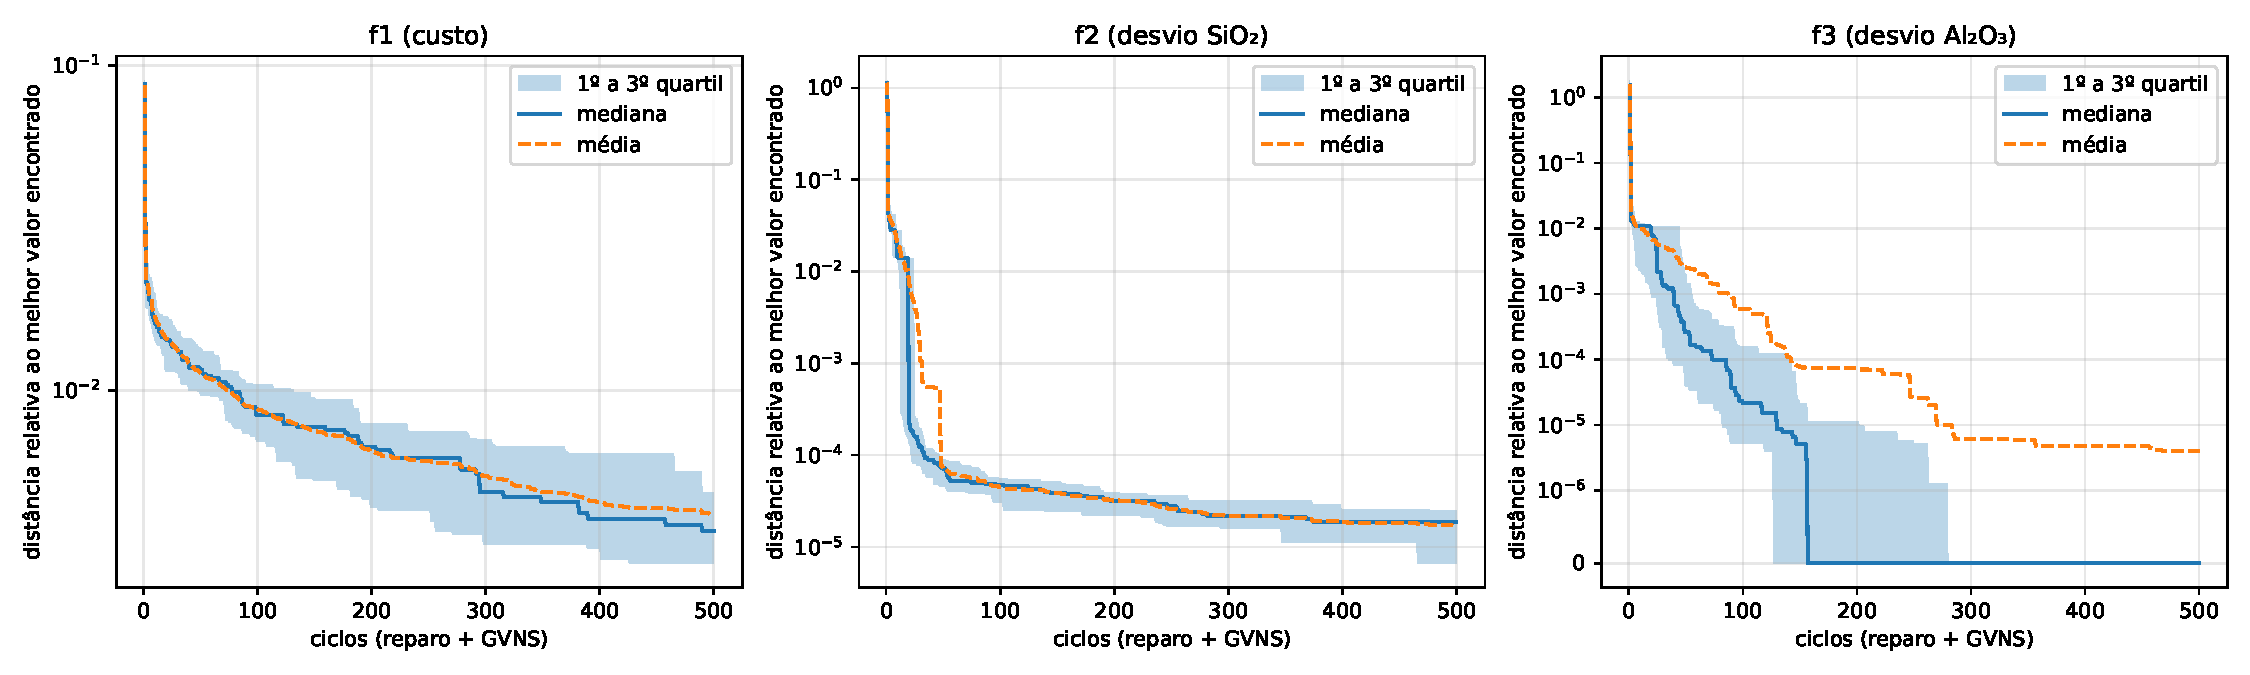
\includegraphics[width=\textwidth]{parada_convergencia.pdf}
\caption{Distância relativa ao melhor valor encontrado em função dos ciclos, em 30 execuções de 500 ciclos por objetivo: mediana, média e faixa entre o primeiro e o terceiro quartis. Eixo vertical em escala logarítmica, com trecho linear junto ao zero.}
\label{fig:parada}
\end{figure*}

\begin{table}[htbp]
\caption{Distância relativa média ao melhor valor encontrado e fração das execuções que o atingem, por orçamento de ciclos}
\centering
\begin{tabular}{r r r r r}
\toprule
\textbf{$C$} & \textbf{$f_1$} & \textbf{$f_2$} & \textbf{$f_3$} & \textbf{$f_3$ no melhor} \\
\midrule
50 & $1{,}14\%$ & $7{,}0\times10^{-5}$ & $2{,}6\times10^{-3}$ & 7\% \\
100 & $0{,}88\%$ & $4{,}5\times10^{-5}$ & $5{,}9\times10^{-4}$ & 20\% \\
200 & $0{,}65\%$ & $3{,}2\times10^{-5}$ & $7{,}4\times10^{-5}$ & 57\% \\
300 & $0{,}55\%$ & $2{,}2\times10^{-5}$ & $6{,}1\times10^{-6}$ & 80\% \\
500 & $0{,}42\%$ & $1{,}7\times10^{-5}$ & $4{,}0\times10^{-6}$ & 87\% \\
\bottomrule
\end{tabular}
\label{tab:parada}
\end{table}

Os três objetivos convergem em ritmos diferentes. Em $f_3$, a maior parte das execuções atinge o melhor valor entre 150 e 300 ciclos; com 50 ciclos, só 7\% o atingiam. Em $f_2$, a curva forma um patamar a partir de cerca de 300 ciclos. Em $f_1$, a melhora continua até 500 ciclos, mas em ritmo decrescente: de 300 para 500 ciclos, a distância média cai apenas 0{,}13 ponto percentual, com cerca de 67\% a mais de esforço. Também foi avaliada a parada após $K$ ciclos consecutivos sem melhora, com $K$ de 10 a 150. Para o mesmo número médio de ciclos, ela ficou ligeiramente pior que o orçamento fixo em $f_1$ e equivalente em $f_2$ e $f_3$; como também torna o esforço de cada execução variável, o que dificulta comparar configurações e abordagens, foi mantido o orçamento fixo. Adotou-se, portanto, $C=300$ ciclos, ponto em que $f_2$ e $f_3$ já estão no patamar e o ganho adicional em $f_1$ não compensa o custo, considerando também as 115 chamadas da execução final multiobjetivo.

O melhor valor encontrado nessas execuções foi R\$~59{,}36 milhões para $f_1$, 2{,}3726305~pp$^2$ para $f_2$ e 1{,}4199714~pp$^2$ para $f_3$. Na comparação com a referência exata, $f_1$ tem ótimo provado de R\$~59{,}34 milhões, a 0{,}03\% do melhor valor da GVNS. Em $f_2$ e $f_3$, o Gurobi não provou a otimalidade em cerca de quatro horas de execução, mas sua melhor solução coincide com a melhor da GVNS, com intervalo de otimalidade final (MIP Gap) de $3{,}8\times10^{-5}$ e $4{,}8\times10^{-5}$, respectivamente.

\subsection{Resultados para $f_1$}

A Tabela~\ref{tab:res_f1} apresenta o custo da melhor solução viável obtida em cada uma das cinco execuções finais, com $C=300$ ciclos e $\phi=0{,}25$, além do número de avaliações, dos nós visitados na enumeração de $N_3$ e do tempo medido. Todas as execuções terminaram com soluções viáveis, e o reparo encontrou solução admissível no primeiro ciclo em todas elas.

\begin{table}[htbp]
\caption{Resultados das cinco execuções para $f_1$ (custo)}
\centering
\small\setlength{\tabcolsep}{2.8pt}
\begin{tabular}{c c r r r r}
\toprule
\textbf{Exec.} & \textbf{Semente} & \textbf{$f_1$ (R\$ mi)} & \textbf{Avaliações} & \textbf{Nós $N_3$} & \textbf{Tempo (s)} \\
\midrule
1 & 2027 & 59{,}90 & 2\,032\,952 & 9\,041\,275 & 576{,}1 \\
2 & 2028 & 59{,}70 & 1\,781\,448 & 7\,197\,077 & 482{,}4 \\
3 & 2029 & 60{,}00 & 1\,883\,803 & 10\,327\,626 & 611{,}8 \\
4 & 2030 & 59{,}60 & 1\,636\,057 & 5\,279\,871 & 379{,}3 \\
5 & 2031 & \textbf{59{,}44} & 1\,805\,648 & 6\,265\,072 & 442{,}6 \\
\midrule
\multicolumn{2}{l}{Mínimo} & 59{,}44 & & & \\
\multicolumn{2}{l}{Média} & 59{,}73 & & & \\
\multicolumn{2}{l}{Desvio padrão} & 0{,}23 & & & \\
\multicolumn{2}{l}{Máximo} & 60{,}00 & & & \\
\bottomrule
\end{tabular}
\label{tab:res_f1}
\end{table}

O menor custo encontrado foi R\$~59{,}44 milhões (execução 5), 0{,}17\% acima do ótimo provado de R\$~59{,}34 milhões; a média das cinco execuções ficou 0{,}65\% acima dele. A diferença entre a melhor e a pior execução foi de R\$~560 mil, cerca de 0{,}9\% do menor custo. Em $f_1$, o número de nós visitados em $N_3$ é várias vezes maior que o de avaliações: os cortes descartam a maior parte das receitas antes de completá-las, mas a vizinhança continua grande, porque muitas reconstruções preservam a viabilidade.

\subsection{Resultados para $f_2$}

A Tabela~\ref{tab:res_f2} apresenta os resultados da minimização do desvio quadrático de SiO$_2$.

\begin{table}[htbp]
\caption{Resultados das cinco execuções para $f_2$ (desvio de SiO$_2$)}
\centering
\small\setlength{\tabcolsep}{2.8pt}
\begin{tabular}{c c l r r r}
\toprule
\textbf{Exec.} & \textbf{Semente} & \textbf{$f_2$ (pp$^2$)} & \textbf{Avaliações} & \textbf{Nós $N_3$} & \textbf{Tempo (s)} \\
\midrule
1 & 12027 & \textbf{2{,}37267} & 9\,711\,306 & 273\,210 & 736{,}1 \\
2 & 12028 & 2{,}37268 & 9\,142\,885 & 260\,640 & 708{,}7 \\
3 & 12029 & 2{,}37271 & 8\,980\,555 & 227\,299 & 703{,}5 \\
4 & 12030 & 2{,}37272 & 8\,210\,399 & 219\,872 & 663{,}5 \\
5 & 12031 & 2{,}37269 & 8\,573\,662 & 228\,995 & 685{,}8 \\
\midrule
\multicolumn{2}{l}{Mínimo} & 2{,}37267 & & & \\
\multicolumn{2}{l}{Média} & 2{,}37269 & & & \\
\multicolumn{2}{l}{Desvio padrão} & $2{,}0\times10^{-5}$ & & & \\
\multicolumn{2}{l}{Máximo} & 2{,}37272 & & & \\
\bottomrule
\end{tabular}
\label{tab:res_f2}
\end{table}

As cinco execuções chegaram a valores praticamente iguais: a diferença entre a melhor e a pior é de $4{,}9\times10^{-5}$~pp$^2$, e a melhor fica a $1{,}7\times10^{-5}$ em termos relativos da melhor solução conhecida, 2{,}3726305~pp$^2$. Ao contrário de $f_1$, em $f_2$ o número de avaliações é muito maior que o de nós de $N_3$: perto de boas soluções de $f_2$ há poucas receitas que preservam a qualidade, e o esforço se concentra em $N_1$ e $N_2$.

\subsection{Resultados para $f_3$}

A Tabela~\ref{tab:res_f3} apresenta os resultados da minimização do desvio quadrático de Al$_2$O$_3$.

\begin{table}[htbp]
\caption{Resultados das cinco execuções para $f_3$ (desvio de Al$_2$O$_3$)}
\centering
\small\setlength{\tabcolsep}{2.8pt}
\begin{tabular}{c c l r r r}
\toprule
\textbf{Exec.} & \textbf{Semente} & \textbf{$f_3$ (pp$^2$)} & \textbf{Avaliações} & \textbf{Nós $N_3$} & \textbf{Tempo (s)} \\
\midrule
1 & 22027 & 1{,}42003 & 12\,617\,320 & 195\,551 & 823{,}6 \\
2 & 22028 & 1{,}41997 & 11\,463\,115 & 179\,454 & 797{,}6 \\
3 & 22029 & 1{,}41998 & 11\,156\,301 & 204\,246 & 779{,}1 \\
4 & 22030 & \textbf{1{,}41997} & 12\,292\,628 & 192\,010 & 812{,}5 \\
5 & 22031 & 1{,}41998 & 11\,806\,191 & 191\,298 & 800{,}7 \\
\midrule
\multicolumn{2}{l}{Mínimo} & 1{,}41997 & & & \\
\multicolumn{2}{l}{Média} & 1{,}41999 & & & \\
\multicolumn{2}{l}{Desvio padrão} & $2{,}4\times10^{-5}$ & & & \\
\multicolumn{2}{l}{Máximo} & 1{,}42003 & & & \\
\bottomrule
\end{tabular}
\label{tab:res_f3}
\end{table}

As execuções 2 e 4 atingiram 1{,}4199714~pp$^2$, o mesmo valor da melhor solução do Gurobi, e as demais ficaram a menos de $6\times10^{-5}$~pp$^2$ dele. Com um orçamento de 50 ciclos, apenas 7\% das execuções do estudo do critério de parada atingiam esse valor (Tabela~\ref{tab:parada}).

\subsection{Curvas de Convergência}

As Figuras~\ref{fig:conv_f1}, \ref{fig:conv_f2} e~\ref{fig:conv_f3} sobrepõem as cinco curvas de convergência de cada objetivo. Cada curva mostra o melhor valor viável encontrado até o momento em função do número de avaliações de soluções candidatas. Como a solução construtiva pode violar os limites de qualidade, cada curva começa apenas quando o reparo encontra a primeira solução viável; as avaliações gastas no reparo são contabilizadas no eixo horizontal.

\begin{figure}[htbp]
\centering
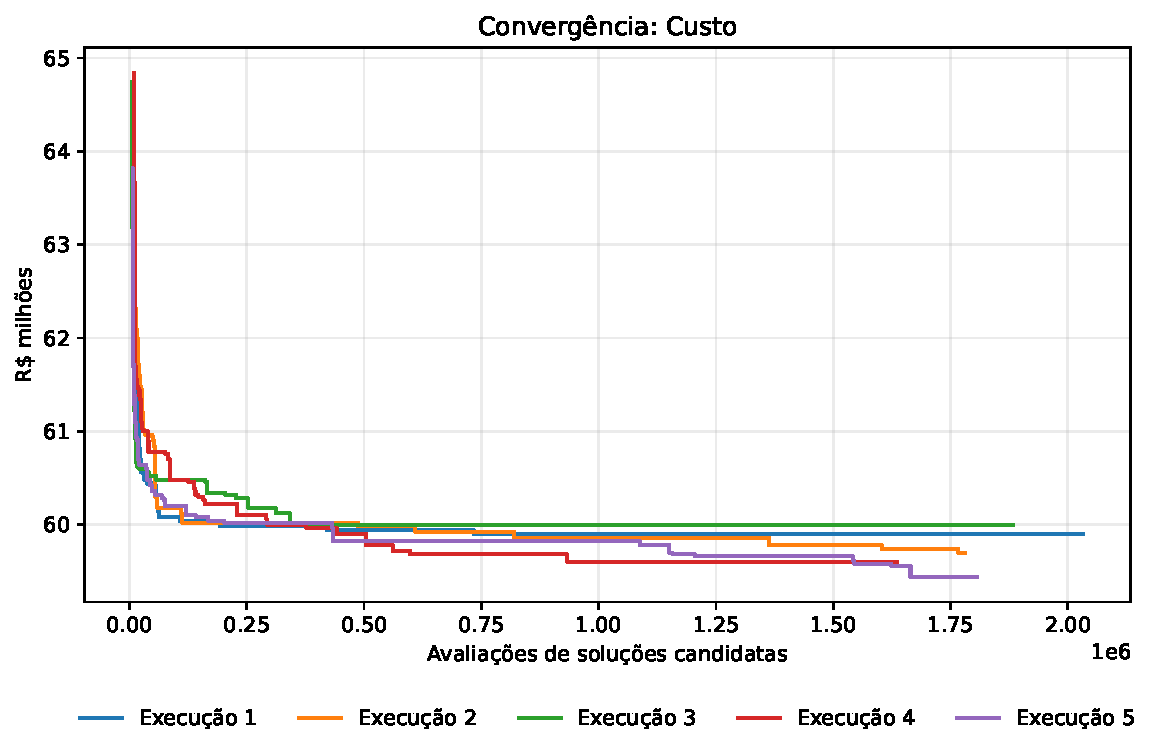
\includegraphics[width=\columnwidth]{convergencia_f1.pdf}
\caption{Curvas de convergência das cinco execuções para $f_1$ (custo).}
\label{fig:conv_f1}
\end{figure}

\begin{figure}[htbp]
\centering
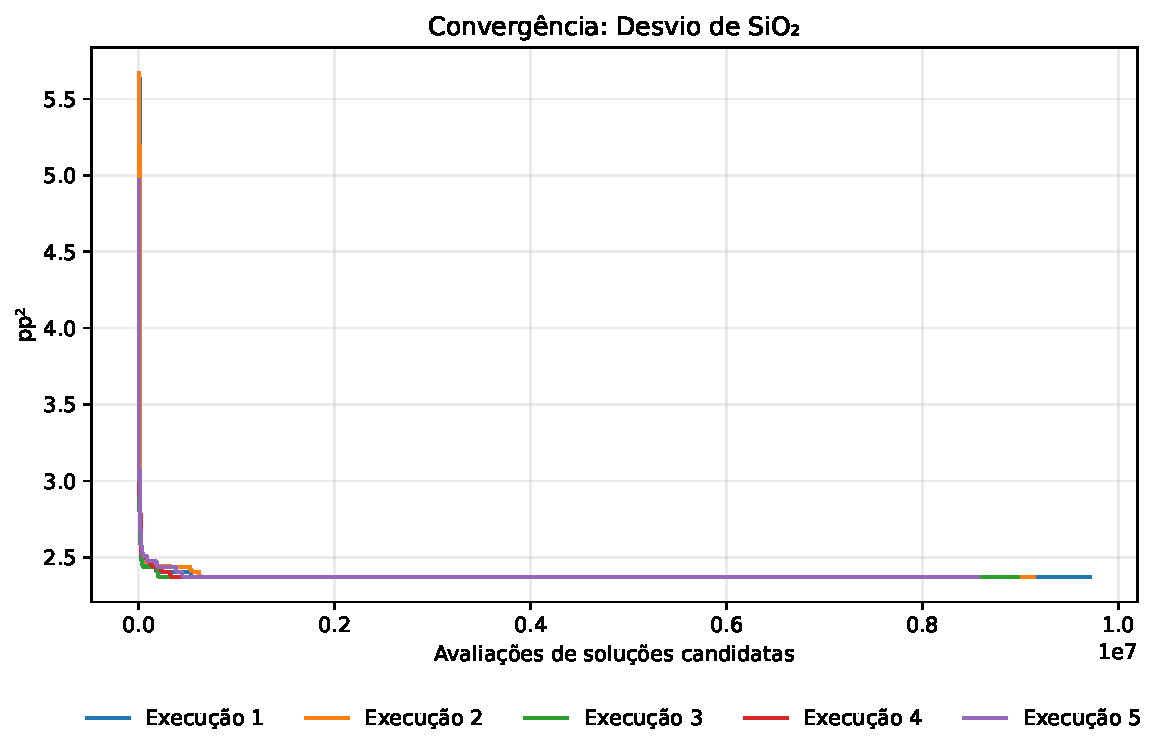
\includegraphics[width=\columnwidth]{convergencia_f2.pdf}
\caption{Curvas de convergência das cinco execuções para $f_2$ (desvio de SiO$_2$).}
\label{fig:conv_f2}
\end{figure}

\begin{figure}[htbp]
\centering
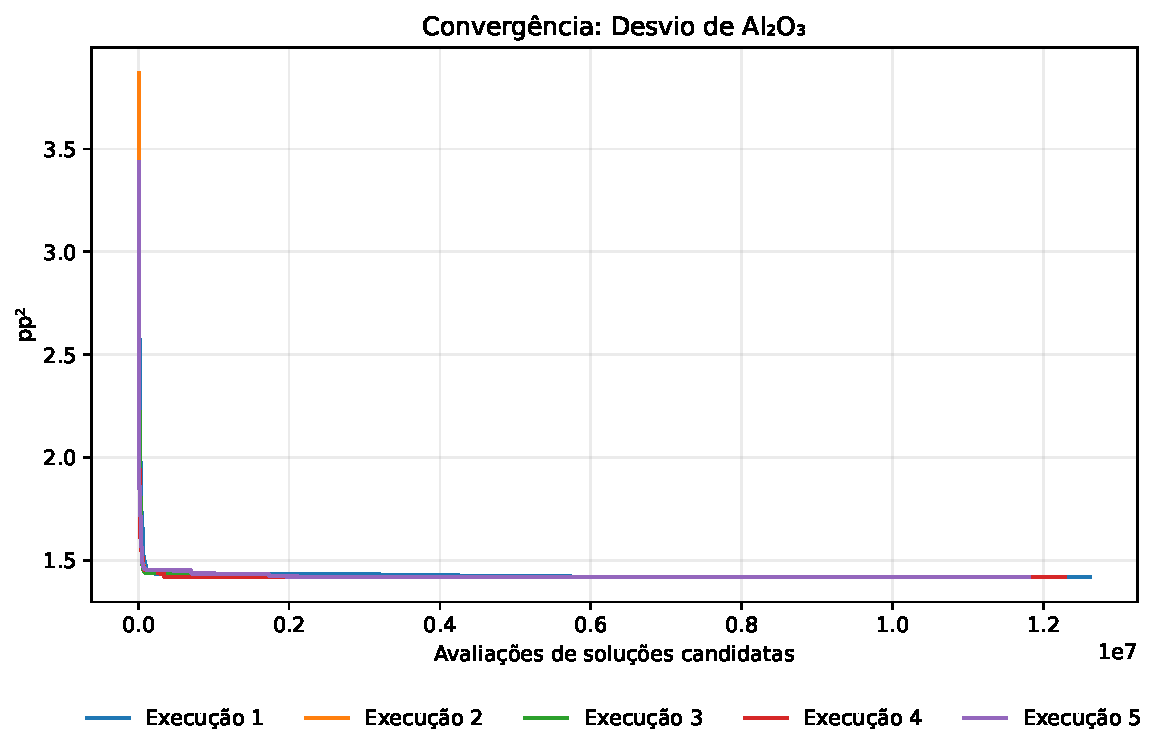
\includegraphics[width=\columnwidth]{convergencia_f3.pdf}
\caption{Curvas de convergência das cinco execuções para $f_3$ (desvio de Al$_2$O$_3$).}
\label{fig:conv_f3}
\end{figure}

Nos três objetivos, a maior parte da melhoria ocorre no início da busca. Em $f_1$, as execuções continuam melhorando em saltos pequenos e espaçados até o fim do orçamento e terminam em patamares diferentes, como já indicava o estudo do critério de parada. Em $f_2$ e $f_3$, as curvas se estabilizam cedo e convergem para praticamente o mesmo valor.

\subsection{Melhores Soluções Encontradas}

As Figuras~\ref{fig:melhor_f1}, \ref{fig:melhor_f2} e~\ref{fig:melhor_f3} representam a melhor solução obtida para cada objetivo. Cada linha corresponde a uma pilha e cada coluna a um minério; o número em cada célula é a quantidade de caminhões daquele minério na pilha, e a intensidade da cor acompanha esse número. A linha horizontal separa as pilhas do Sinter~1 (P1--P5) das do Sinter~2 (P6--P10). À direita, são apresentados os teores de SiO$_2$ e Al$_2$O$_3$ resultantes em cada pilha.

A Tabela~\ref{tab:comparacao} avalia cada uma dessas soluções nos três objetivos.

\begin{table}[htbp]
\caption{Valores dos três objetivos nas melhores soluções de cada otimização}
\centering
\begin{tabular}{l r r r}
\toprule
\textbf{Otimizado} & \textbf{$f_1$ (R\$ mi)} & \textbf{$f_2$ (pp$^2$)} & \textbf{$f_3$ (pp$^2$)} \\
\midrule
$f_1$ & \textbf{59{,}44} & 6{,}801 & 6{,}762 \\
$f_2$ & 63{,}44 & \textbf{2{,}373} & 3{,}763 \\
$f_3$ & 65{,}82 & 6{,}271 & \textbf{1{,}420} \\
\bottomrule
\end{tabular}
\label{tab:comparacao}
\end{table}

A tabela evidencia o conflito entre os objetivos. A solução de menor custo tem os maiores desvios de qualidade; reduzir o desvio de Al$_2$O$_3$ ao mínimo encontrado custa R\$~6{,}38 milhões a mais (10{,}7\%). Nenhuma das três soluções é melhor que as outras em todos os objetivos, o que motiva a abordagem multiobjetivo da Seção~\ref{sec:multi}.

Na solução de menor custo (Figura~\ref{fig:melhor_f1}), o teor de SiO$_2$ de P2 e P4 é 6{,}200\%, no máximo permitido pelo Sinter~1, e as demais pilhas desse sinter ficam entre 6{,}180\% e 6{,}186\%. As pilhas do Sinter~2 ficam entre 6{,}453\% e 6{,}494\%, perto do máximo de 6{,}5\%. O custo baixo é acompanhado de misturas próximas dos limites de sílica, enquanto os alvos químicos continuam distantes.

Nas soluções de $f_2$ e $f_3$ (Figuras~\ref{fig:melhor_f2} e~\ref{fig:melhor_f3}), os teores não atingem os valores-alvo. Na solução de $f_2$, o SiO$_2$ varia de 5{,}880\% a 6{,}126\%, acima dos alvos de 5{,}55\% (Sinter~1) e 5{,}50\% (Sinter~2). Na de $f_3$, o Al$_2$O$_3$ varia de 1{,}500\% a 1{,}607\% no Sinter~1 (alvo de 1{,}25\%) e de 1{,}880\% a 1{,}984\% no Sinter~2 (alvo de 1{,}5\%), crescendo com a massa da pilha dentro de cada sinter. A disponibilidade limitada e a ausência de ponderação por massa podem contribuir para esse padrão, mas essa interpretação não constitui uma demonstração causal.


\section{Otimização Multiobjetivo}\label{sec:multi}

\subsection{Normalização Fixa}
Seja $X$ o conjunto de planos que satisfazem todas as restrições físicas
originais. Utilizamos as melhores soluções das cinco execuções isoladas
para formar a matriz de resultados cruzados da Tabela~\ref{tab:payoff}.
\begin{table}[htbp]
\centering\small
\caption{Referências empíricas da Entrega 1.}
\label{tab:payoff}
\begin{tabular}{lrrr}\toprule
Referência & $f_1$ (R\$ mi) & $f_2$ (pp$^2$) & $f_3$ (pp$^2$)\\\midrule
Menor custo & 59,44 & 6,80062097 & 6,76186898\\
Menor SiO$_2$ & 63,44 & 2,37267124 & 3,76293269\\
Menor Al$_2$O$_3$ & 65,82 & 6,27074879 & 1,41997141\\\bottomrule
\end{tabular}
\end{table}
Para cada objetivo $q\in\{1,2,3\}$, definimos $a_q$ e $b_q$ como o menor
e o maior valor da coluna correspondente nessa matriz:
\begin{equation}
\bar f_q(x)=\frac{f_q(x)-a_q}{b_q-a_q}.
\end{equation}
São escalas empíricas, não provas exatas e não cortamos
valores abaixo de 0 nem acima de 1. O arquivo \texttt{normalizacao.json}
guarda valores completos, receitas, sementes e hash dos dados. Ao carregar,
o programa reavalia as receitas e confere os extremos. Uma escala nula ou
um arquivo de dados diferente provoca erro; a normalização não muda durante
os experimentos.

\subsection{Soma Ponderada}
A abordagem resolve
\begin{equation}
\min_{x\in X} g_w(x)=\sum_{q=1}^{3}w_q\bar f_q(x),
\qquad w_q\geq 0,\quad\sum_{q=1}^{3}w_q=1.
\end{equation}
A grade inclui $(1/3,1/3,1/3)$, as três permutações de $(0{,}6,0{,}2,0{,}2)$
e as três permutações de $(0{,}5,0{,}5,0)$. A primeira configuração equilibra
os indicadores normalizados; as demais exploram prioridades individuais e
compromissos entre pares. A Soma
Ponderada pode não alcançar regiões não suportadas de uma fronteira não
convexa~\cite{blank_deb2020}; a heurística tampouco garante o mínimo global de cada combinação.

\subsection{Método $\varepsilon$-restrito}
Usamos a formulação convencional de $\varepsilon$-restrito~\cite{gams_eps},
mantendo o custo como objetivo e limitando os dois desvios agregados:
\begin{align}
\min_{x\in X}\quad &\bar f_1(x)\\
\text{sujeito a}\quad &\bar f_2(x)\leq\varepsilon_2,\\
&\bar f_3(x)\leq\varepsilon_3.
\end{align}
A grade é o produto cartesiano $\{0{,}10;0{,}25;0{,}50;1{,}00\}^2$, totalizando
16 pares, escolhida como descrito adiante. Por exemplo, $\varepsilon_2=0{,}25$ impõe
$f_2\leq a_2+0{,}25(b_2-a_2)$; não significa um teor de 0,25\%.
Para $\varepsilon_q=1$, o limite adicional é $b_q$, o máximo empírico
da coluna de referência. Mantêm-se também os limites físicos de cada pilha.
A admissibilidade ativa exige as restrições físicas e os dois $\varepsilon$,
com tolerância absoluta de $10^{-10}$ nos valores normalizados.

\subsection{Adaptação da GVNS e do Reparo}
As duas abordagens utilizam \texttt{solve\_scalar}; a interface mono-objetivo
também chama essa mesma rotina. O operador, a perturbação, a VND e a regra
de aceitação permanecem os mesmos, mudando apenas o valor escalar e a
admissibilidade ativa. Na Soma Ponderada, o reparo minimiza a violação física.
No $\varepsilon$-restrito, utiliza
\begin{equation}
\begin{split}
V_\varepsilon(x)={}&V_{\mathrm{fis}}(x)+\max(0,\bar f_2(x)-\varepsilon_2)\\
&+\max(0,\bar f_3(x)-\varepsilon_3),
\end{split}
\end{equation}
desprezando somente excessos numéricos de até $10^{-10}$ por limite.
Essa medida guia exclusivamente o reparo e não é somada ao custo.
Não utilizamos termo aumentado ou desempate lexicográfico; a filtragem
posterior remove as soluções dominadas encontradas.
O atendimento dos $\varepsilon$ é verificado no registro da melhor solução,
na perturbação e na VND. A reconstrução $N_3$ mantém sua definição física,
mas não garante, por si só, os dois limites agregados.

Os cortes de $N_3$ descritos na Seção~\ref{sec:gvns} valem para qualquer
critério que seja uma combinação com pesos não negativos dos três objetivos.
Como $\bar f_q$ é uma função linear de $f_q$ somada a uma constante, a Soma Ponderada equivale, a menos de uma
constante, a minimizar $\sum_q w_q f_q/(b_q-a_q)$; no $\varepsilon$-restrito,
o critério é $f_1/(b_1-a_1)$ mais uma constante. Em ambos os casos, o
limitante da variação do critério na pilha reconstruída é a soma ponderada
dos limitantes de cada objetivo. No $\varepsilon$-restrito, o corte usa só o
custo: receitas que não reduzem o custo são descartadas, e o atendimento dos
$\varepsilon$ continua verificado na avaliação de cada vizinho.

\paragraph{Política única e obrigatória de partida}
Todas as chamadas mono-objetivo, Soma Ponderada e $\varepsilon$-restrito
executam a mesma função \texttt{construct(case)} da Entrega 1: distribuição
dos mínimos obrigatórios e preenchimento por preço. Para os mesmos dados,
a construção bruta é determinística e idêntica em todas as abordagens.
As receitas de referência são utilizadas exclusivamente para a normalização;
não são usadas como partida das buscas.

Cada chamada repara essa construção conforme suas restrições ativas.
Na Soma Ponderada e no mono-objetivo, são as restrições físicas; no
$\varepsilon$-restrito, são as físicas e os dois $\varepsilon$.
Como o reparo utiliza a semente da chamada e critérios de admissibilidade
que podem diferir, sua saída pode ser diferente. Assim, a igualdade da
construção não implica identidade do plano admissível que inicia a GVNS.
Os registros identificam a partida como \texttt{construcao}.

O reparo segue a política da Seção~\ref{sec:construtiva}: recomeça da
construção a cada $R=100$ ciclos sem solução admissível e divide com a GVNS
o orçamento de $C$ ciclos da chamada. Uma configuração $\varepsilon$-restrita
pode esgotar o orçamento no reparo, seja por não admitir solução ou por a
heurística não conseguir encontrá-la. Nesse caso, a chamada é registrada como
falha de reparo, nenhum ponto inviável é exportado como solução e o lote
prossegue. A falha não prova impossibilidade matemática da configuração.

\subsection{Rodadas, Configurações e Reprodução}
Uma rodada de cada abordagem percorre toda a sua grade. Cinco rodadas
correspondem a 35 chamadas escalares para Soma Ponderada e 80 para
$\varepsilon$-restrito. Cada chamada reinicia a GVNS e utiliza o mesmo orçamento de
$C=\Cparada$ ciclos da Entrega~1, sem teto de candidatos, nós ou tempo em $N_3$.
Essa organização operacional das cinco execuções deve ser distinguida dos
valores da grade, que não são fixados pelo enunciado.

Para rodada $r$ e configuração de índice $c$ começando em um, utilizamos
\begin{equation}
\mathrm{semente}=2026+d+1000r+c,
\end{equation}
com $d=100000$ na Soma Ponderada e $d=200000$ no $\varepsilon$-restrito.
A fórmula é uma convenção reproduzível, não um parâmetro de qualidade.
As receitas, sementes, curvas, falhas e configurações ficam salvas por
chamada. Repetir o comando retoma somente as chamadas pendentes; a
retomada rejeita mudanças nos dados, código, normalização ou parâmetros.
A quantidade de processos pode mudar sem alterar as sementes das chamadas.

\subsection{Dominância e Visualizações}
Para todos os objetivos minimizados, $u$ domina $v$ quando
\begin{equation}
f_q(u)\leq f_q(v)\quad\forall q,
\qquad\exists q:\ f_q(u)<f_q(v).
\end{equation}
A implementação usa tolerâncias absolutas de $10^{-6}$ R\$ para custo e
$10^{-10}$ pp$^2$ para cada desvio. Comparamos os valores completos antes de
arredondar e filtramos a união das cinco rodadas separadamente por abordagem.
Composições idênticas são reunidas, preservando todas as origens; receitas
diferentes com os mesmos objetivos permanecem disponíveis para a etapa
multicritério. Exportamos também conjuntos não dominados por rodada.

Os seis gráficos são gerados somente com Matplotlib, em PDF: $f_1\times f_2$,
$f_1\times f_3$ e $f_2\times f_3$ para cada abordagem. As cores identificam
rodadas; uma receita compartilhada é desenhada nas cores das suas origens.
A filtragem é feita em três dimensões, nunca novamente em cada projeção.
São conjuntos não dominados entre as soluções encontradas, não uma prova
da fronteira exata.

Para comparar as abordagens, usamos duas medidas complementares de
Zitzler e Thiele~\cite{zitzler1999}. O hipervolume é o volume do espaço
normalizado dominado pelo conjunto e limitado pelo ponto de referência
$(1{,}1;\,1{,}1;\,1{,}1)$, comum às duas abordagens; quanto maior, melhor a
combinação de convergência e espalhamento. A cobertura $\mathcal{C}(A,B)$ é a
fração dos pontos de $B$ dominados por algum ponto de $A$ ou iguais a ele nos
três objetivos. Calculamos também quantos pontos de cada abordagem permanecem
no conjunto não dominado da união das duas e, para avaliar a variabilidade,
o hipervolume do conjunto de cada rodada. As duas abordagens têm números de
chamadas diferentes (35 e 80), o que deve ser considerado na comparação.

\subsection{Escolha das Grades}
A grade de $\varepsilon$ precisa incluir valores pequenos, pois limites normalizados apenas a partir de 0{,}25 deixariam sem exploração o trecho da fronteira entre o melhor desvio isolado e um quarto da faixa de cada desvio, justamente o de melhor qualidade. Por outro lado, limites muito apertados nos dois desvios ao mesmo tempo podem não admitir solução. Para escolher a grade, foi feito um teste simplificado de uma rodada e 100 ciclos com $\varepsilon_2,\varepsilon_3\in\{0{,}05;0{,}10;0{,}25;0{,}50;1{,}00\}$ e os sete pesos da Soma Ponderada, com referências de normalização preliminares.

No teste, os pares com $\varepsilon=0{,}05$ ou $0{,}10$ alcançaram a região de alta qualidade da fronteira, por exemplo $f_2\approx2{,}58$~pp$^2$ com custo de R\$~63{,}7 milhões e $f_3\approx1{,}66$~pp$^2$ com R\$~64{,}8 milhões, que nenhum par com $\varepsilon\geq0{,}25$ atingiu. Os pares $(0{,}05;0{,}05)$, $(0{,}05;0{,}10)$ e $(0{,}10;0{,}05)$, que restringem os dois desvios ao mesmo tempo, esgotaram o orçamento no reparo sem solução admissível. Adotou-se, por isso, a grade $\{0{,}10;0{,}25;0{,}50;1{,}00\}^2$, com 16 pares, que cobre a região de alta qualidade sem os pares inviáveis no teste. A execução final tem, assim, 35 chamadas de Soma Ponderada e 80 de $\varepsilon$-restrito.

\subsection{Resultados da Soma Ponderada}
\begin{figure*}[!t]
\centering
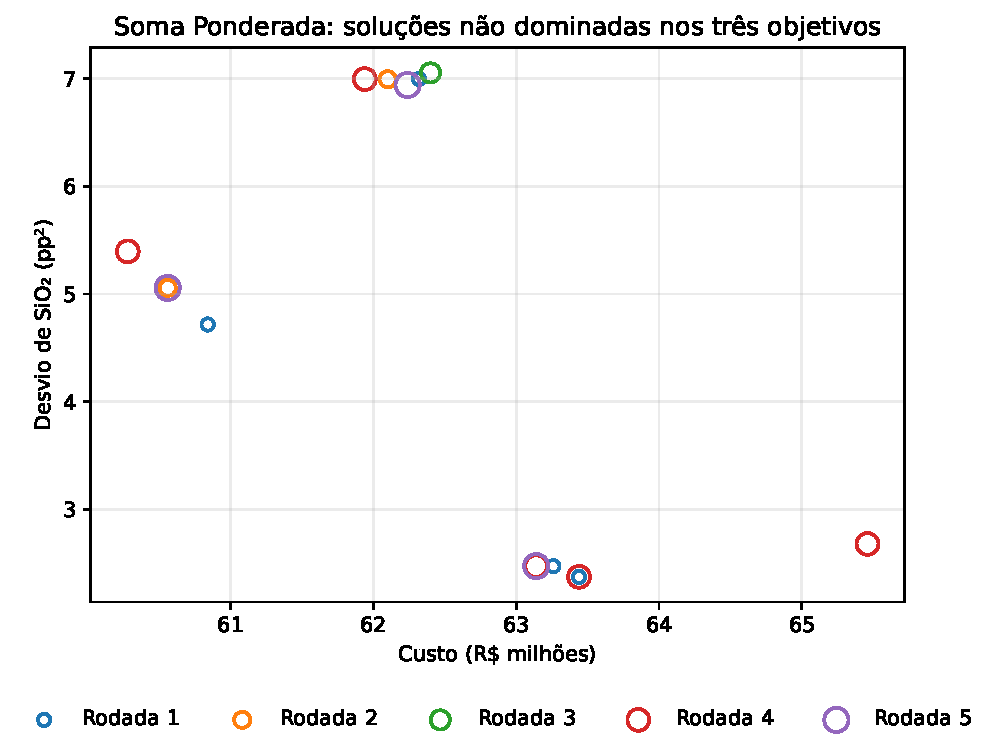
\includegraphics[width=0.32\textwidth]{soma_f1_f2.pdf}\hfill
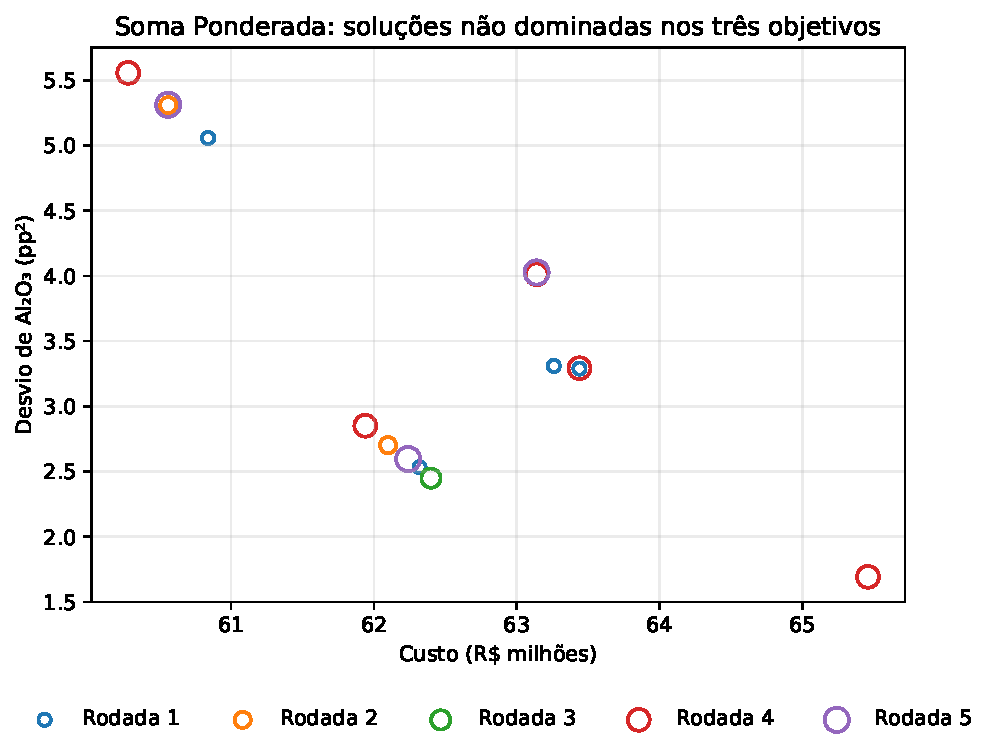
\includegraphics[width=0.32\textwidth]{soma_f1_f3.pdf}\hfill
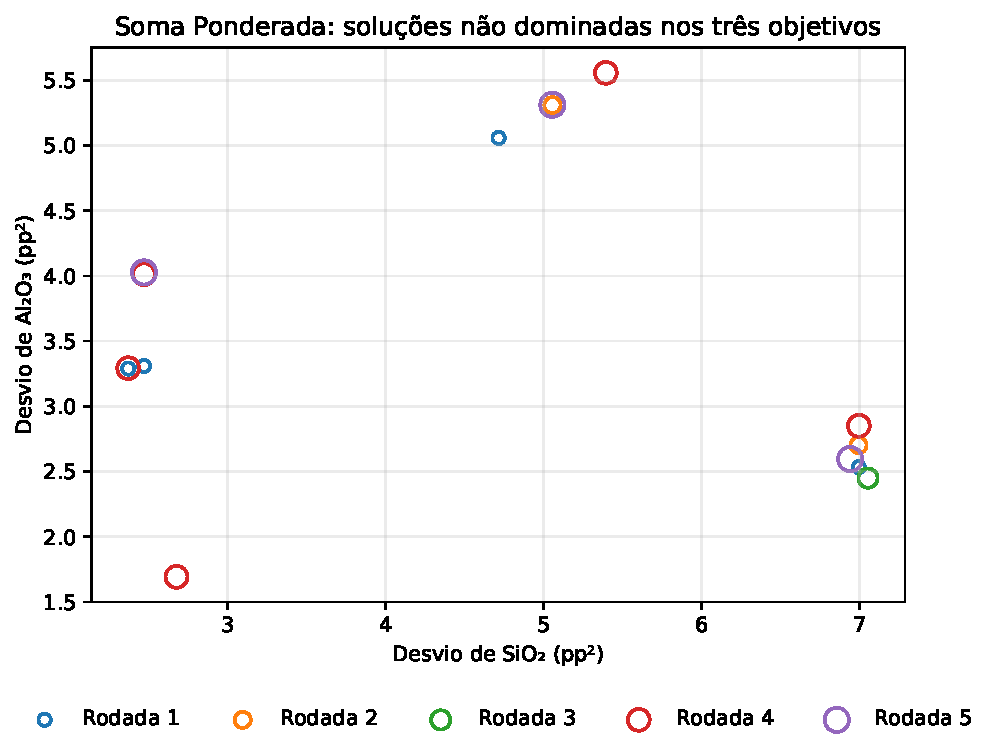
\includegraphics[width=0.32\textwidth]{soma_f2_f3.pdf}
\caption{Soma Ponderada: projeções $f_1\times f_2$, $f_1\times f_3$ e $f_2\times f_3$ das receitas não dominadas nos três objetivos, reunidas das cinco rodadas. As cores identificam a rodada de origem; uma receita encontrada em mais de uma rodada aparece com marcadores sobrepostos.}
\label{fig:proj_soma}
\end{figure*}

As 35 chamadas da Soma Ponderada terminaram com soluções admissíveis, todas com o reparo resolvido no primeiro ciclo. Após a filtragem nos três objetivos, restaram 15 receitas não dominadas, cujas projeções aparecem na Figura~\ref{fig:proj_soma}.

As soluções se concentram em cinco grupos, cada um associado a um vetor de pesos. Os pesos que priorizam o custo produzem as receitas mais baratas, entre R\$~60{,}28 e R\$~60{,}84 milhões, com desvios altos de SiO$_2$ e de Al$_2$O$_3$. A combinação entre custo e alumina leva a custos entre R\$~61{,}94 e R\$~62{,}40 milhões, com $f_3$ entre 2{,}45 e 2{,}85~pp$^2$, mas com $f_2$ acima do maior valor da matriz de referência ($\bar f_2>1$), pois o peso da sílica é nulo. Os pesos que dão destaque à sílica, inclusive o vetor equilibrado, convergem para receitas com $f_2$ próximo do mínimo isolado e custo entre R\$~63{,}14 e R\$~63{,}44 milhões. O peso que prioriza a alumina gera a receita de menor $f_3$ do conjunto, 1{,}69~pp$^2$, ao custo de R\$~65{,}46 milhões. As receitas do vetor que combina sílica e alumina com peso nulo no custo ficaram próximas às do vetor da alumina e foram dominadas por elas.

Entre as rodadas, cada vetor de pesos produziu cinco receitas distintas, mas com valores escalares muito próximos: a maior diferença relativa entre a melhor e a pior rodada de um mesmo vetor foi de cerca de 1\%, no vetor do custo. As rodadas, portanto, alcançaram as mesmas regiões do espaço de objetivos, como mostra a sobreposição das cores na Figura~\ref{fig:proj_soma}. O hipervolume dos conjuntos de cada rodada variou entre 0{,}542 e 0{,}566, e o da união das cinco rodadas foi 0{,}584.

O conjunto obtido deixa lacunas entre os grupos, por exemplo entre R\$~60{,}84 e R\$~61{,}94 milhões, e nenhum vetor produziu receitas com os desvios de SiO$_2$ e de Al$_2$O$_3$ ambos em níveis intermediários. Esse comportamento é esperado na Soma Ponderada: cada vetor de pesos conduz a busca a um único ponto, e regiões não suportadas da fronteira não são alcançadas por nenhuma combinação de pesos~\cite{blank_deb2020}. O resultado indica também que a grade de sete vetores é grosseira para descrever a fronteira; vetores intermediários poderiam preencher parte das lacunas, ao custo de mais chamadas.

\subsection{Resultados do Método $\varepsilon$-restrito}
\begin{figure*}[!t]
\centering
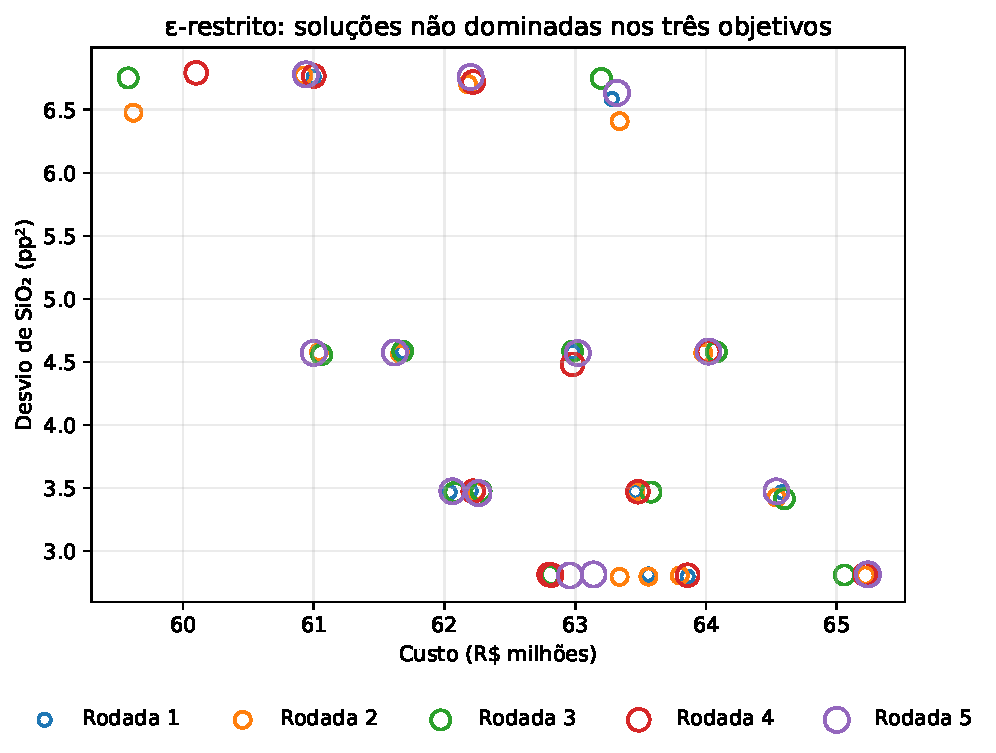
\includegraphics[width=0.32\textwidth]{epsilon_f1_f2.pdf}\hfill
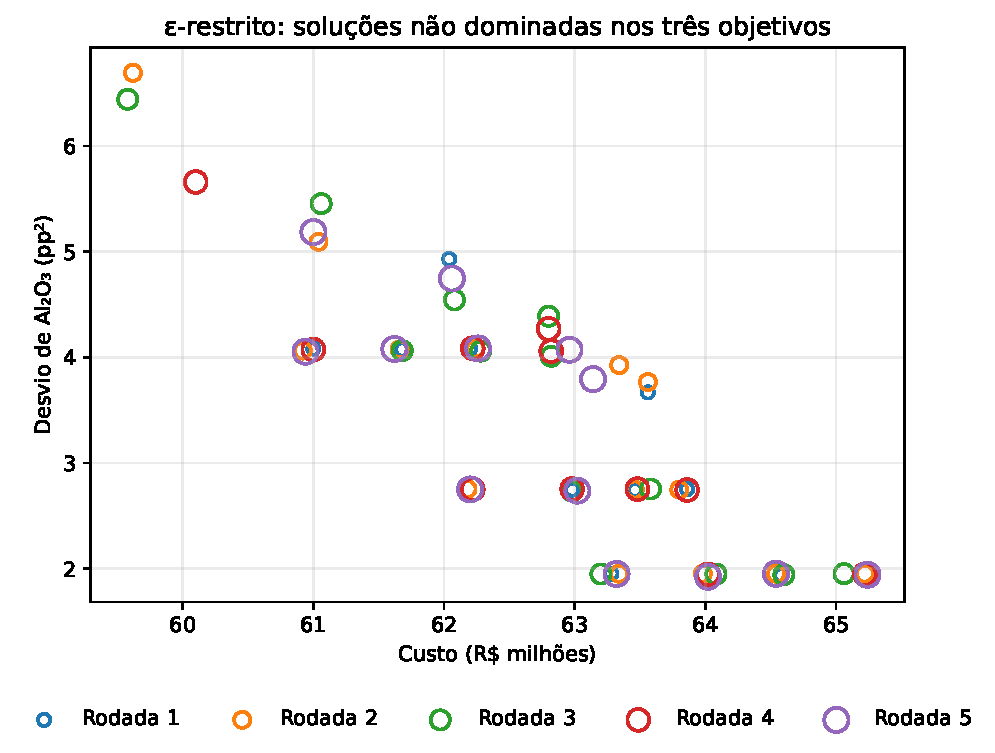
\includegraphics[width=0.32\textwidth]{epsilon_f1_f3.pdf}\hfill
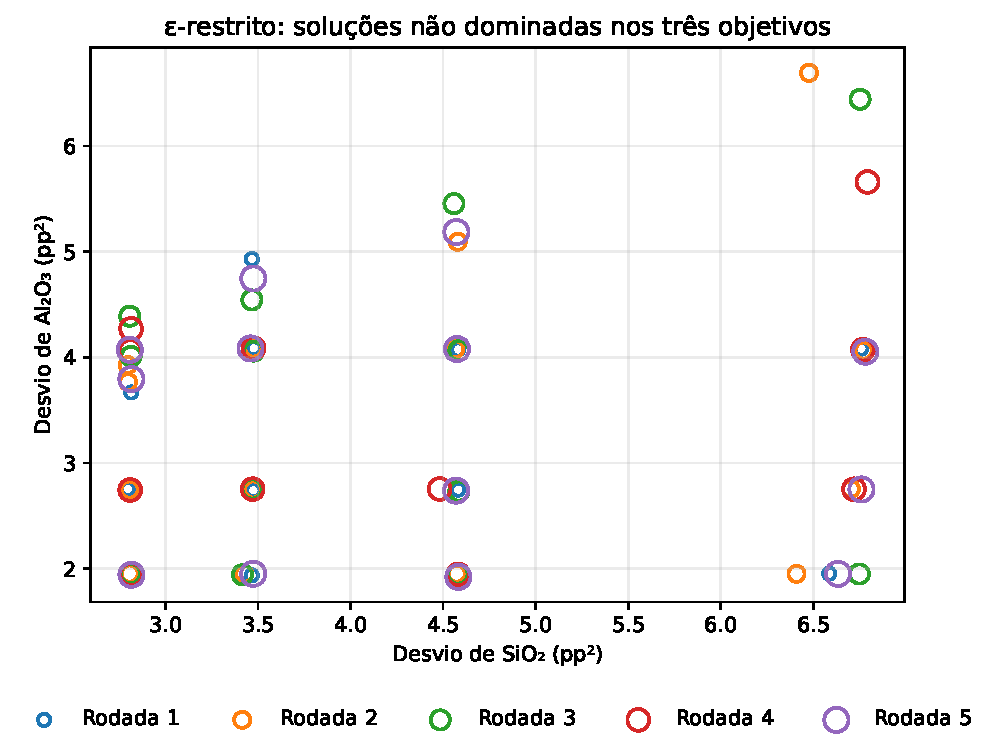
\includegraphics[width=0.32\textwidth]{epsilon_f2_f3.pdf}
\caption{$\varepsilon$-restrito: projeções $f_1\times f_2$, $f_1\times f_3$ e $f_2\times f_3$ das receitas não dominadas nos três objetivos, reunidas das cinco rodadas. As cores identificam a rodada de origem.}
\label{fig:proj_eps}
\end{figure*}

As 80 chamadas do $\varepsilon$-restrito terminaram com soluções admissíveis; nenhuma esgotou o orçamento no reparo. Após a filtragem nos três objetivos, restaram 61 receitas não dominadas, apresentadas na Figura~\ref{fig:proj_eps}. Elas cobrem custos de R\$~59{,}58 a R\$~65{,}24 milhões, desvios de SiO$_2$ de 2{,}80 a 6{,}79~pp$^2$ e desvios de Al$_2$O$_3$ de 1{,}92 a 6{,}69~pp$^2$.

Em todas as chamadas, ao menos um dos limites $\varepsilon$ ficou ativo na solução final, isto é, o desvio normalizado terminou a menos de 0{,}02 do seu limite. Esse comportamento é esperado: minimizar o custo empurra a solução até o limite de qualidade permitido, e cada par de $\varepsilon$ produz, assim, um ponto distinto da fronteira. Por isso, ao contrário da Soma Ponderada, o $\varepsilon$-restrito distribui as soluções de forma regular pelo espaço de objetivos, seguindo a grade. O custo cresce à medida que os limites ficam mais apertados: de R\$~59{,}58 milhões no par $(1{,}00;1{,}00)$ até R\$~65{,}06 milhões no par $(0{,}10;0{,}10)$.

As rodadas alcançaram as mesmas regiões. Para cada par de $\varepsilon$, a diferença entre o maior e o menor custo das cinco rodadas ficou abaixo de 1{,}3\%, e o hipervolume do conjunto de cada rodada variou entre 0{,}627 e 0{,}640. As maiores diferenças ocorreram nos pares com $\varepsilon_2=0{,}10$ e $\varepsilon_3\geq0{,}50$, em que o limite de sílica é apertado e o de alumina é folgado; uma explicação possível, não verificada, é que essa combinação admite muitas receitas de custo próximo, entre as quais a busca termina em pontos diferentes.


\subsection{Comparação entre as Abordagens}

\begin{figure*}[!t]
\centering
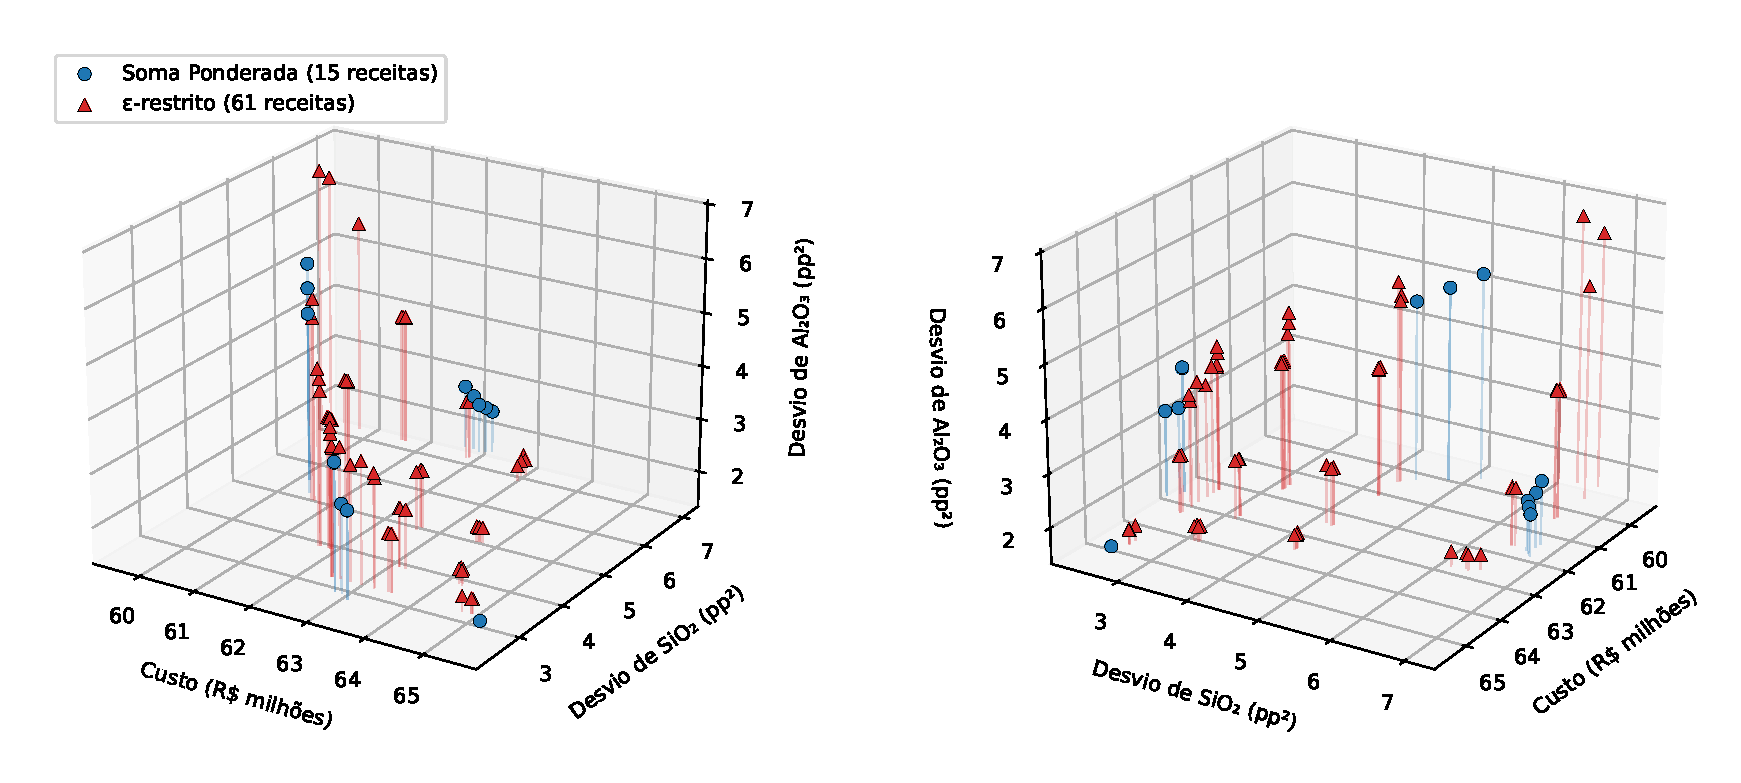
\includegraphics[width=\textwidth]{frente_3d.pdf}
\caption{Receitas não dominadas da Soma Ponderada (círculos) e do $\varepsilon$-restrito (triângulos) no espaço dos três objetivos, em duas vistas. As linhas verticais ligam cada ponto ao menor desvio de Al$_2$O$_3$ do gráfico, para indicar a altura.}
\label{fig:frente_3d}
\end{figure*}

A Tabela~\ref{tab:comparacao_multi} resume as medidas de comparação, e a Figura~\ref{fig:frente_3d} mostra os dois conjuntos no espaço dos três objetivos.

\begin{table}[htbp]
\caption{Comparação entre os conjuntos não dominados das duas abordagens}
\centering
\begin{tabular}{l r r}
\toprule
\textbf{Medida} & \textbf{Soma Pond.} & \textbf{$\varepsilon$-restrito} \\
\midrule
Chamadas & 35 & 80 \\
Receitas não dominadas & 15 & 61 \\
Hipervolume normalizado & 0{,}584 & 0{,}655 \\
Cobertura sobre a outra, $\mathcal{C}$ & 0{,}049 & 0 \\
Pontos na união não dominada & 15 & 58 \\
Menor $f_1$ (R\$ mi) & 60{,}28 & 59{,}58 \\
Menor $f_2$ (pp$^2$) & 2{,}373 & 2{,}796 \\
Menor $f_3$ (pp$^2$) & 1{,}692 & 1{,}924 \\
\bottomrule
\end{tabular}
\label{tab:comparacao_multi}
\end{table}

O $\varepsilon$-restrito obteve maior hipervolume (0{,}655 contra 0{,}584) e muito mais receitas não dominadas, distribuídas por toda a superfície de compromisso, enquanto a Soma Ponderada concentrou as soluções em cinco grupos. A diferença no número de chamadas (80 contra 35) explica parte dessa vantagem, mas não a distribuição: mesmo vetores de pesos distintos levaram a Soma Ponderada às mesmas regiões, ao passo que cada par de $\varepsilon$ fixa um nível de qualidade diferente.

As duas abordagens são, porém, complementares. Nenhuma receita da Soma Ponderada é dominada pelas do $\varepsilon$-restrito, e todas as 15 permanecem no conjunto não dominado da união das duas, que tem 73 receitas. Em parte, isso ocorre porque a Soma Ponderada alcançou os extremos de alta qualidade: desvio de SiO$_2$ de 2{,}373~pp$^2$ e de Al$_2$O$_3$ de 1{,}692~pp$^2$, abaixo do que permite o menor $\varepsilon$ da grade, 0{,}10, que corresponde a $f_2\leq2{,}815$~pp$^2$ e $f_3\leq1{,}954$~pp$^2$. O $\varepsilon$-restrito, por sua vez, encontrou o menor custo da etapa, R\$~59{,}58 milhões, e preencheu o interior da fronteira que a Soma Ponderada não alcança.

O principal compromisso observado é entre custo e qualidade. Partindo da receita mais barata, reduzir os dois desvios exige substituir minérios baratos e de teores elevados, como M13, M15 e M17, por minérios mais caros, como M1, M3 e M6. No conjunto da união, levar os dois desvios ao nível do par $(0{,}10;0{,}10)$ custa cerca de R\$~5{,}5 milhões a mais que a receita de menor custo. Entre os dois desvios, o conflito é menor: há receitas com ambos baixos, mas elas ficam no extremo caro da fronteira. As receitas da união formam o conjunto de alternativas para a etapa de decisão multicritério.

\section{Decisão Multicritério}\label{sec:decisao}

\subsection{Alternativas e Critérios}\label{sec:criterios}

As alternativas são as receitas da união dos conjuntos não dominados da Soma Ponderada (15 receitas) e do $\varepsilon$-restrito (61 receitas). Cada receita é reavaliada na instância, e os objetivos recalculados precisam coincidir com os gravados na etapa anterior. As duas abordagens não encontraram nenhuma receita em comum, e três receitas do $\varepsilon$-restrito são dominadas por outras da união. Restam 73 alternativas, nomeadas A01 a A73 em ordem crescente de custo.

Os critérios são os três objetivos, $f_1$, $f_2$ e $f_3$, e a homogeneidade da receita das pilhas de um mesmo equipamento, $H$, sugerida no enunciado. Seja $I_s=\{i\in I \mid s(i)=s\}$ o conjunto das pilhas do equipamento $s$ e $N_i=\sum_{j\in J}x_{ij}$ o número de caminhões da pilha $i$. A receita da pilha é a fração de caminhões de cada minério, e a receita comum do equipamento é a fração calculada sobre todas as suas pilhas:
\begin{align}
r_{ij} &= \frac{x_{ij}}{N_i}, \qquad
\bar r_{sj} = \frac{\sum_{i\in I_s}x_{ij}}{\sum_{i\in I_s}N_i}, \\
H_s &= \frac{1}{|I_s|}\sum_{i\in I_s}\sum_{j\in J}\left|r_{ij}-\bar r_{sj}\right|, \qquad
H = \frac{1}{|S|}\sum_{s\in S}H_s.
\end{align}
O valor $H/2$ é a fração dos caminhões de uma pilha que precisaria trocar de minério para igualar a receita comum. O critério vale zero quando todas as pilhas de cada equipamento têm a mesma proporção de minérios e é minimizado. Nas 73 alternativas, $H$ varia de 0{,}734 a 1{,}057.

O enunciado exige que o critério extra seja conflitante com os demais. Com $H$ incluído, nenhuma das 73 alternativas passa a ser dominada. Adotamos a homogeneidade por ter leitura direta na operação do pátio.

\subsection{Pesos e Entrevista com o Decisor}\label{sec:pesos}

Neste trabalho somos a unidade de decisão, mas os pesos não foram arbitrados diretamente. Estruturamos uma entrevista em que as perguntas descrevem o problema, e não os parâmetros dos métodos, e obtivemos os pesos e os limiares a partir das respostas. As subseções seguintes descrevem o instrumento, a aplicação, o tratamento das respostas e o resultado.

\subsubsection{Instrumento}

O instrumento é um formulário eletrônico com cinco seções (Tabela~\ref{tab:formulario}), cujo texto completo está no Apêndice~A. Quatro decisões orientam as perguntas.

Primeiro, cada critério é apresentado pela melhoria do pior ao melhor valor existente entre as 73 alternativas: custo de R\$~65{,}5 a R\$~59{,}6 milhões, desvio típico de cada pilha em relação ao alvo de 0{,}84 a 0{,}49~pp na sílica e de 0{,}82 a 0{,}41~pp na alumina, e receita de cada pilha diferindo da receita comum em 53\% a 37\% dos caminhões. Assim, a importância declarada se refere à faixa de variação do critério, e não ao critério em abstrato, cuidado destacado nas aulas~\cite{aula10}. O desvio típico é a raiz do desvio quadrático dividido pelo número de pilhas, e a fração de caminhões é $H/2$; as duas grandezas são mais fáceis de interpretar do que $f_2$, $f_3$ e $H$.

Segundo, as comparações usam a escala verbal de Saaty, com os níveis moderadamente, fortemente, muito fortemente e extremamente mais, registrados com os valores 3, 5, 7 e 9. Os valores pares da escala não são oferecidos. Terceiro, cada comparação tem nove opções simétricas: o primeiro critério do par pode valer mais (valores positivos), os dois podem valer o mesmo (valor 1) ou o segundo pode valer mais (valores negativos). Quarto, os $n(n-1)/2=6$ pares dos quatro critérios são todos perguntados, o que permite medir a consistência dos julgamentos. As perguntas sobre os limiares trazem exemplos numéricos na unidade de cada critério.

\begin{table}[htbp]
\caption{Seções do formulário da entrevista}
\centering
\small
\begin{tabular}{c p{0.58\columnwidth} c}
\toprule
\textbf{Seção} & \textbf{Conteúdo} & \textbf{Perguntas} \\
\midrule
1 & Apresentação do problema e dos quatro critérios & 0 \\
2 & Melhoria de maior valor e de menor valor & 2 \\
3 & Intensidade da preferência em cada um dos 6 pares de critérios & 6 \\
4 & Maior piora tolerada e fração mínima da importância & 2 \\
5 & Observações livres (opcional) & 1 \\
\bottomrule
\end{tabular}
\label{tab:formulario}
\end{table}

\subsubsection{Aplicação}

Um profissional da Cassotis, empresa que propôs o case, respondeu ao formulário no papel de decisor. A Tabela~\ref{tab:entrevista} reúne as respostas.

\begin{table}[htbp]
\caption{Respostas da entrevista. Nas comparações, o primeiro critério do par foi o preferido, e a intensidade segue a escala de Saaty: 3, moderadamente; 7, muito fortemente; 9, extremamente mais}
\centering
\small
\begin{tabular}{p{0.62\columnwidth} c}
\toprule
\textbf{Pergunta} & \textbf{Resposta} \\
\midrule
Melhoria de maior valor & Custo \\
Melhoria de menor valor & $H$ \\
Maior piora tolerada (fração da faixa) & 25\% \\
Fração mínima da importância & 80\% \\
Custo contra sílica & 7 \\
Custo contra alumina & 7 \\
Custo contra homogeneidade & 9 \\
Sílica contra alumina & 3 \\
Sílica contra homogeneidade & 7 \\
Alumina contra homogeneidade & 7 \\
\bottomrule
\end{tabular}
\label{tab:entrevista}
\end{table}

\subsubsection{Tratamento das respostas}

Cada comparação vira um julgamento $a_{ij}$ da matriz de comparação par a par $A$ dos critérios, na escala de Saaty: o valor $n>0$ significa que o critério $i$ vale $n$ vezes o critério $j$ e dá $a_{ij}=n$, o valor $-n$ dá $a_{ij}=1/n$, e a igualdade dá $a_{ij}=1$. A matriz é completada por reciprocidade, $a_{ji}=1/a_{ij}$, e o vetor de pesos $w$ é o autovetor principal de $A$, normalizado para somar 1 (Seção~\ref{sec:ahp}).

A consistência é verificada de duas formas. O quociente de consistência QC deve ser de no máximo 0{,}10, limite adotado nas aulas; se for maior, o decisor revê os julgamentos que mais se afastam da consistência. Além disso, o critério apontado como de maior valor deve ter o maior peso, e o de menor valor, o menor. Das respostas sobre os limiares, a maior piora tolerada define o veto declarado, em fração da faixa, e a fração mínima da importância define o apoio mínimo declarado; os dois são valores de referência para $\tau_d$ e $\tau_c$ (Seção~\ref{sec:electre}).

\subsubsection{Resultado}

As respostas da Cassotis formam a matriz $A$, na ordem custo, SiO$_2$, Al$_2$O$_3$ e $H$:
\begin{equation}
A=\begin{bmatrix}
1 & 7 & 7 & 9\\
1/7 & 1 & 3 & 7\\
1/7 & 1/3 & 1 & 7\\
1/9 & 1/7 & 1/7 & 1
\end{bmatrix},
\end{equation}
com vetor de pesos $w=(0{,}671;\ 0{,}186;\ 0{,}110;\ 0{,}033)$. O custo tem o maior peso e a homogeneidade, o menor, como o respondente indicou nas perguntas sobre a melhoria de maior e de menor valor. O QC, porém, é 0{,}20, o dobro do limite.

A inconsistência vem do teto da escala de Saaty, e não de um julgamento isolado. O custo vale 7 vezes a sílica, e a sílica vale 7 vezes a homogeneidade, o que implicaria um custo cerca de 49 vezes mais importante que a homogeneidade; a escala, no entanto, termina em 9, e o próprio vetor de pesos indica uma razão de cerca de 20. Nenhuma mudança de um ou dois degraus em um único julgamento traz o QC para 0{,}10 ou menos; a melhor chega a 0{,}14. Enviamos ao respondente uma devolutiva com quatro composições reais entre as 73, a indicação que os pesos produziam e uma pergunta de pontuação sem teto, no formato do método SMART das aulas~\cite{aula10}, mas não houve resposta até o fechamento do trabalho.

Decidimos usar os julgamentos da Cassotis como estão, por virem de quem conhece a operação, e registrar o QC acima do limite como limitação. A análise de sensibilidade acompanha essa decisão com perturbações dos julgamentos que não aumentam a inconsistência. O mesmo vetor $w$ alimenta o ELECTRE~I e o AHP.

Como limitações, a entrevista teve um único respondente, e a ordem das perguntas foi fixa, o que pode influenciar as respostas; não testamos outras ordens.

\subsection{ELECTRE I}\label{sec:electre}

Seguimos a formulação e a notação das aulas~\cite{aula_electre}; o método integra a família descrita por Figueira, Mousseau e Roy~\cite{figueira2005}. Nesta seção, o conjunto $J$ e os índices $j$, $i$ e $k$ designam critérios e alternativas, como nas aulas, e não minérios, pilhas e substâncias. Sejam $a_i$ as alternativas, $c_j(a_i)$ o valor do critério $j$ e $w_j$ seu peso. Como os quatro critérios são de minimização, uma alternativa é melhor que outra no critério quando seu valor é menor. Para cada par $(a_i,a_k)$, os critérios se separam em favoráveis, indiferentes e contrários:
\begin{align}
J^{+}(a_i,a_k) &= \{j\in J \mid c_j(a_i) < c_j(a_k)\},\\
J^{=}(a_i,a_k) &= \{j\in J \mid c_j(a_i) = c_j(a_k)\},\\
J^{-}(a_i,a_k) &= \{j\in J \mid c_j(a_i) > c_j(a_k)\}.
\end{align}
O índice de concordância mede o peso dos critérios que apoiam a afirmação $a_i \mathrel{S} a_k$, e o de discordância mede a maior desvantagem de $a_i$ sobre $a_k$, em fração da amplitude do critério:
\begin{align}
C_{ik} &= \frac{\sum_{j\in J^{+}} w_j + \sum_{j\in J^{=}} w_j}{\sum_{j\in J} w_j},\\
D_{ik} &=
\begin{cases}
0, & J^{-}(a_i,a_k)=\varnothing,\\
\displaystyle\max_{j\in J^{-}(a_i,a_k)} \delta_j\,[c_j(a_i)-c_j(a_k)], & \text{caso contrário,}
\end{cases}\\
\delta_j &= \frac{1}{\max_i c_j(a_i)-\min_i c_j(a_i)}.
\end{align}
A alternativa $a_i$ sobreclassifica $a_k$ quando
\begin{equation}
a_i \mathrel{S} a_k \iff C_{ik}\geq\tau_c \ \text{e}\ D_{ik}\leq\tau_d,
\end{equation}
em que $\tau_c$ é o apoio mínimo e $\tau_d$, o veto. A ordenação retira, nível a nível, as alternativas que nenhuma outra sobreclassifica. Quando duas ou mais alternativas se sobreclassificam em circuito, tratamo-las como uma única classe, pois de outro modo nenhuma delas deixaria de ser sobreclassificada.

As alternativas do primeiro nível são incomparáveis entre si, ou indiferentes quando formam um circuito, e todas seguem para o AHP. Partir esse nível exigiria um desempate arbitrário, que evitamos.

Adotamos $\tau_c=0{,}70$ e $\tau_d=0{,}30$, fixados pelo grupo, como unidade de decisão, antes da resposta do formulário. Os valores declarados pelo respondente, 0{,}80 e 0{,}25, entram como variante na análise de sensibilidade. O apoio de 0{,}70 fica pouco acima do peso do custo, 0{,}671: com apoio até 0{,}65, o custo sozinho basta para sobreclassificar, e o primeiro nível se reduz a uma alternativa; com 0{,}70, o custo precisa de pelo menos mais um critério a favor. Com os valores adotados, o grafo tem 660 relações de sobreclassificação e 10 circuitos, e o primeiro nível tem 4 alternativas. As demais combinações de apoio e veto são testadas na Seção~\ref{sec:sensibilidade}.

\subsection{AHP}\label{sec:ahp}

Também seguimos as aulas~\cite{aula10}, com a formulação de Saaty~\cite{saaty1994}. Cada matriz de comparação $A=[a_{ij}]$ é positiva e recíproca, com $a_{ii}=1$ e $a_{ji}=1/a_{ij}$. O vetor de prioridades $v$, com $\sum_i v_i=1$, é o autovetor principal de $A$:
\begin{equation}
A v=\lambda_{\max} v.
\end{equation}
A consistência dos julgamentos é medida pelo índice $IC=(\lambda_{\max}-n)/(n-1)$ e pelo quociente $QC=IC/ICA$, em que $ICA$ é o índice de consistência aleatório; julgamentos com $QC\leq 0{,}10$ são aceitos. Usamos a tabela de $ICA$ das aulas até $n=10$ (0{,}52 para $n=3$ e 0{,}89 para $n=4$, por exemplo) e, para $n>10$, a média de $IC$ de 20\,000 matrizes recíprocas sorteadas na escala de Saaty, a mesma definição da tabela. A síntese global é
\begin{equation}
g = P\,w,
\end{equation}
em que a coluna $j$ de $P$ reúne as prioridades locais das alternativas no critério $j$.

Nas variações da análise de sensibilidade, até 73 alternativas chegam ao AHP, o que exigiria 2\,628 comparações manuais por critério. Derivamos, por isso, as matrizes entre alternativas dos valores medidos, pela faixa de cada critério. Seja $d_{ik}=[c_j(a_k)-c_j(a_i)]/(\max c_j-\min c_j)$ a vantagem de $a_i$ sobre $a_k$ no critério $j$, em fração da amplitude no conjunto. A intensidade de Saaty é $a_{ik}=1+8d_{ik}$ quando $d_{ik}\geq0$ e $a_{ik}=1/(1+8|d_{ik}|)$ caso contrário, de modo que a melhor alternativa contra a pior vale 9, o extremo da escala. A alternativa mais simples, usar a razão entre os valores medidos, comprime as diferenças de custo (R\$~59{,}6 contra R\$~65{,}5 milhões é uma razão de 1{,}10) e contradiz o sentido dos pesos obtidos na entrevista, que se referem à faixa; ela é testada na análise de sensibilidade. No caso base, o maior quociente de consistência entre as matrizes derivadas é 0{,}054.

\subsection{Encadeamento e Incomparabilidade}

Os dois métodos atuam em sequência. O ELECTRE~I, não compensatório, reduz as 73 alternativas às que nenhuma outra supera; o AHP, compensatório, ordena essas alternativas e indica a recomendada. A incomparabilidade que o ELECTRE~I deixa entre as alternativas do primeiro nível é resolvida pelo AHP, que é, assim, o critério adicional exigido para essa situação, sem desempate extra. Só seria necessária uma regra a mais se o AHP terminasse com margem desprezível entre as duas primeiras, o que não ocorreu no caso base.

\subsection{Resultados da Decisão}\label{sec:resultado_decisao}

\begin{figure*}[!t]
\centering
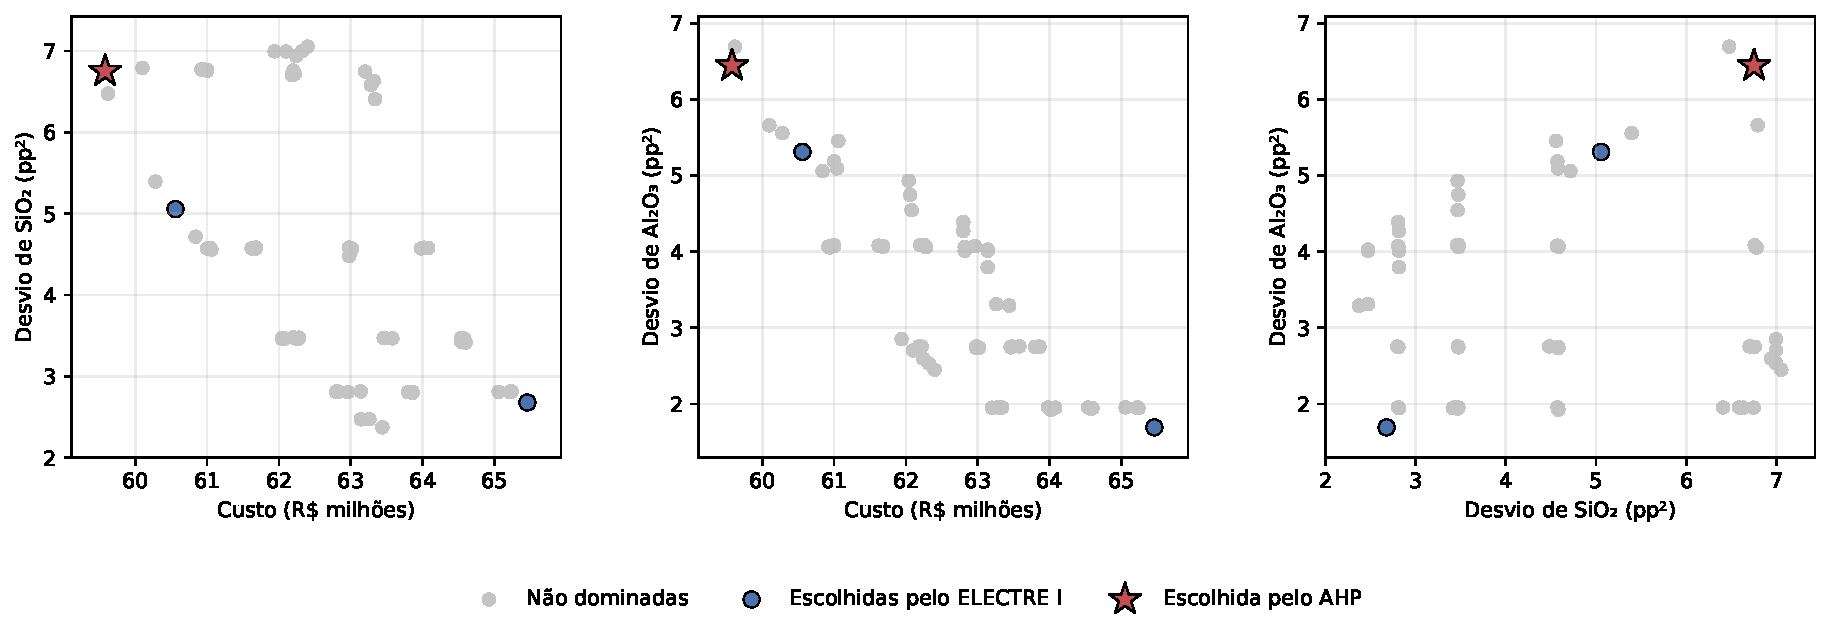
\includegraphics[width=\textwidth]{projecoes_escolha.pdf}
\caption{Projeções das 73 alternativas nos três objetivos, com as quatro escolhidas pelo ELECTRE~I e a escolhida pelo AHP em destaque.}
\label{fig:proj_escolha}
\end{figure*}

\begin{figure*}[!t]
\centering
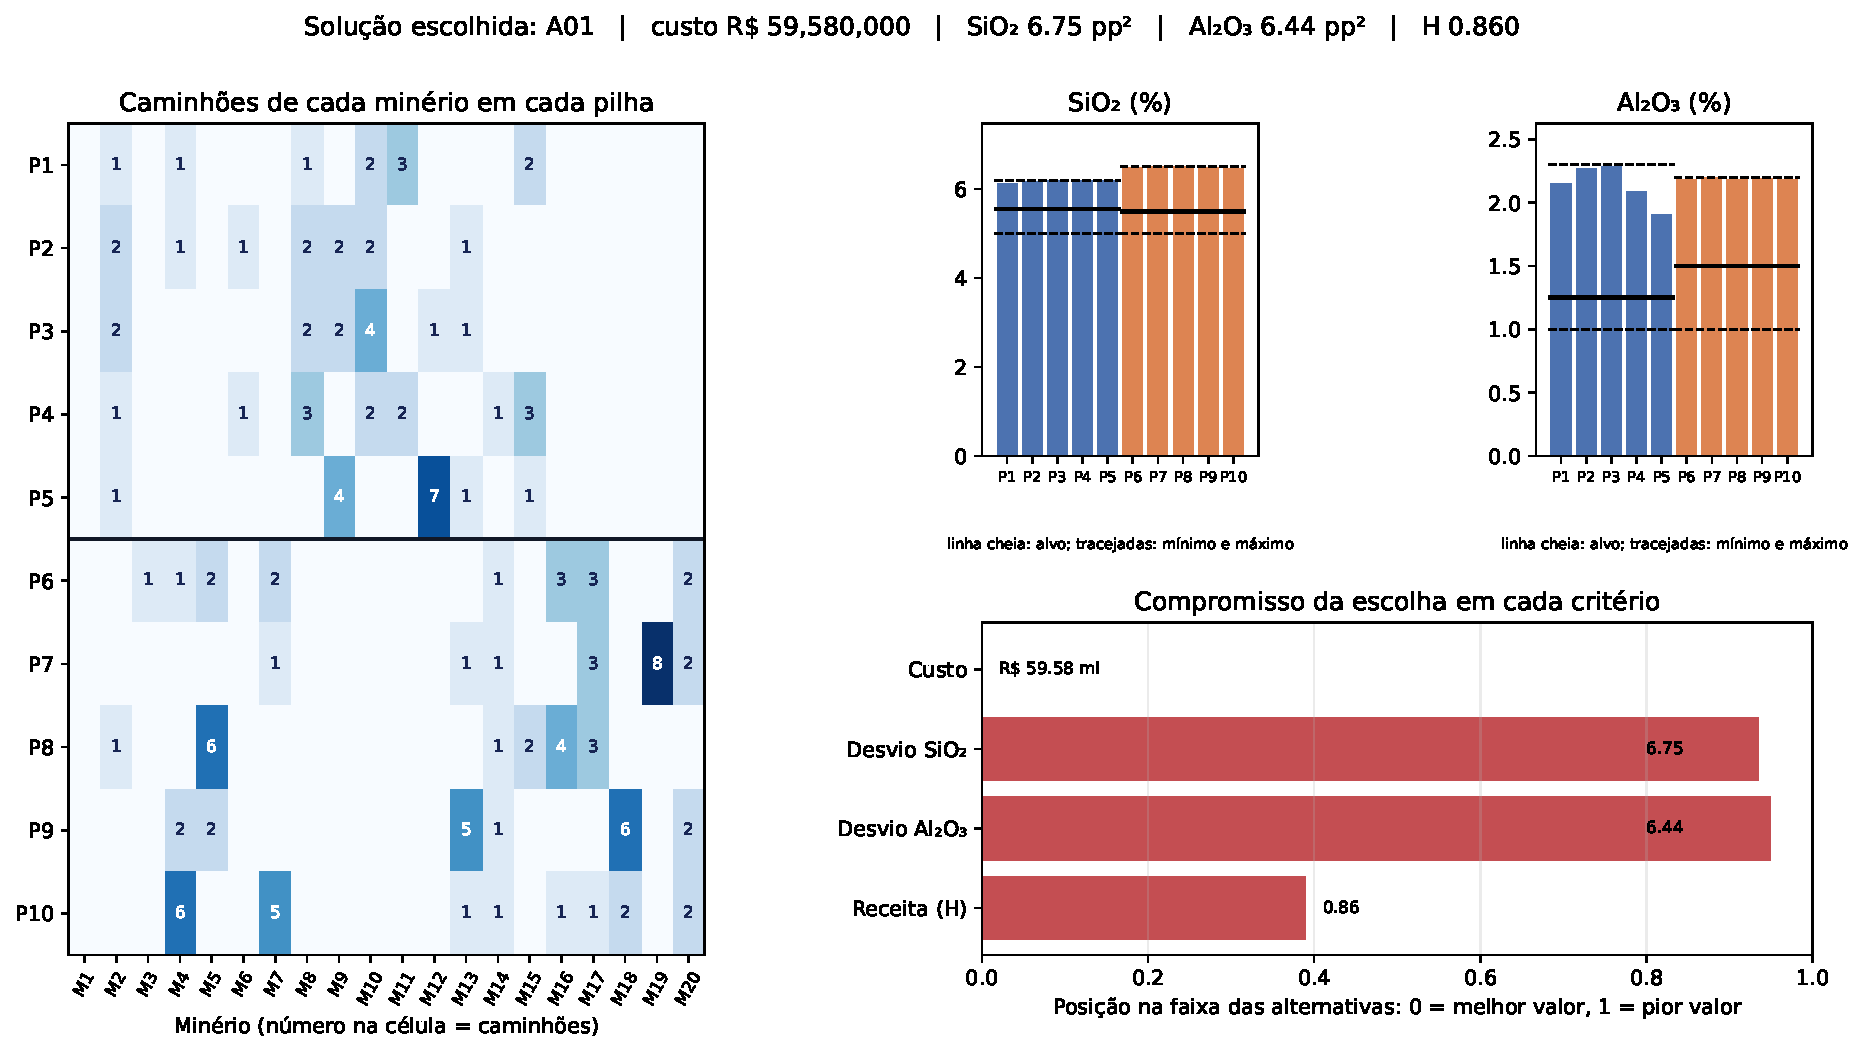
\includegraphics[width=\textwidth]{solucao_final.pdf}
\caption{Solução escolhida: caminhões de cada minério em cada pilha, teor de SiO$_2$ e de Al$_2$O$_3$ de cada pilha com o alvo (linha cheia) e os limites (tracejadas) do equipamento, e posição da solução na faixa de cada critério.}
\label{fig:solucao}
\end{figure*}

O ELECTRE~I escolheu 4 alternativas, e o AHP escolheu entre elas a A01 (Tabela~\ref{tab:nucleo}), com prioridade global 0{,}337, contra 0{,}233 da segunda colocada. O primeiro nível reúne a alternativa de menor custo (A01), a de menor desvio de Al$_2$O$_3$ (A73) e a de receitas mais homogêneas (A05), que forma um circuito com a A06, de objetivos quase iguais. A Figura~\ref{fig:proj_escolha} mostra as alternativas nos três planos de objetivos, e a Tabela~\ref{tab:apendice} do Apêndice~B reúne os critérios de todas as 73.

\begin{table}[htbp]
\caption{Alternativas escolhidas pelo ELECTRE~I, com os critérios e a prioridade global $g$ do AHP. A escolhida pelo AHP está em negrito}
\centering
\small
\begin{tabular}{l r r r r r c}
\toprule
\textbf{Alt.} & $f_1$ (R\$ mi) & $f_2$ & $f_3$ & $H$ & $g$ & \textbf{Pos.} \\
\midrule
\textbf{A01} & \textbf{59{,}58} & \textbf{6{,}75} & \textbf{6{,}44} & \textbf{0{,}860} & \textbf{0{,}337} & \textbf{1} \\
A73 & 65{,}46 & 2{,}68 & 1{,}69 & 0{,}786 & 0{,}233 & 2 \\
A05 & 60{,}56 & 5{,}06 & 5{,}31 & 0{,}734 & 0{,}223 & 3 \\
A06 & 60{,}56 & 5{,}06 & 5{,}31 & 0{,}794 & 0{,}207 & 4 \\
\bottomrule
\end{tabular}
\label{tab:nucleo}
\end{table}

A escolha é um extremo da fronteira. O custo da A01, R\$~59{,}58 milhões, é o menor das 73 alternativas, enquanto os desvios de SiO$_2$ (6{,}75~pp$^2$) e de Al$_2$O$_3$ (6{,}44~pp$^2$) ficam a 94\% e 95\% do caminho entre o melhor e o pior valor dessas alternativas; a homogeneidade, a 39\%. Esse é o compromisso de um peso de 0{,}67 para o custo. Trocar a A01 pela melhor alternativa em Al$_2$O$_3$, a A73, custa R\$~5{,}88 milhões a mais (9{,}9\%) e reduz os desvios de SiO$_2$ em 60\% e de Al$_2$O$_3$ em 74\%; trocá-la pela melhor em SiO$_2$, a A52, custa R\$~3{,}86 milhões a mais (6{,}5\%) e reduz os desvios de SiO$_2$ em 65\% e de Al$_2$O$_3$ em 49\%. Para a homogeneidade, a melhor alternativa, a A05, custa R\$~0{,}98 milhão a mais (1{,}6\%) e ainda reduz os dois desvios.

A Figura~\ref{fig:solucao} mostra uma consequência operacional do custo mínimo: a solução não tem folga em relação à especificação. Todas as pilhas ficam a menos de 0{,}07~pp do limite superior de SiO$_2$, seis das dez ficam a menos de 0{,}02~pp do limite superior de Al$_2$O$_3$ e a pilha~7 está nos dois limites. A solução é viável, mas qualquer variação de teor na chegada dos minérios a levaria para fora da especificação, e o modelo não penaliza essa falta de folga.

\subsection{Análise de Sensibilidade}\label{sec:sensibilidade}

\begin{figure*}[!t]
\centering
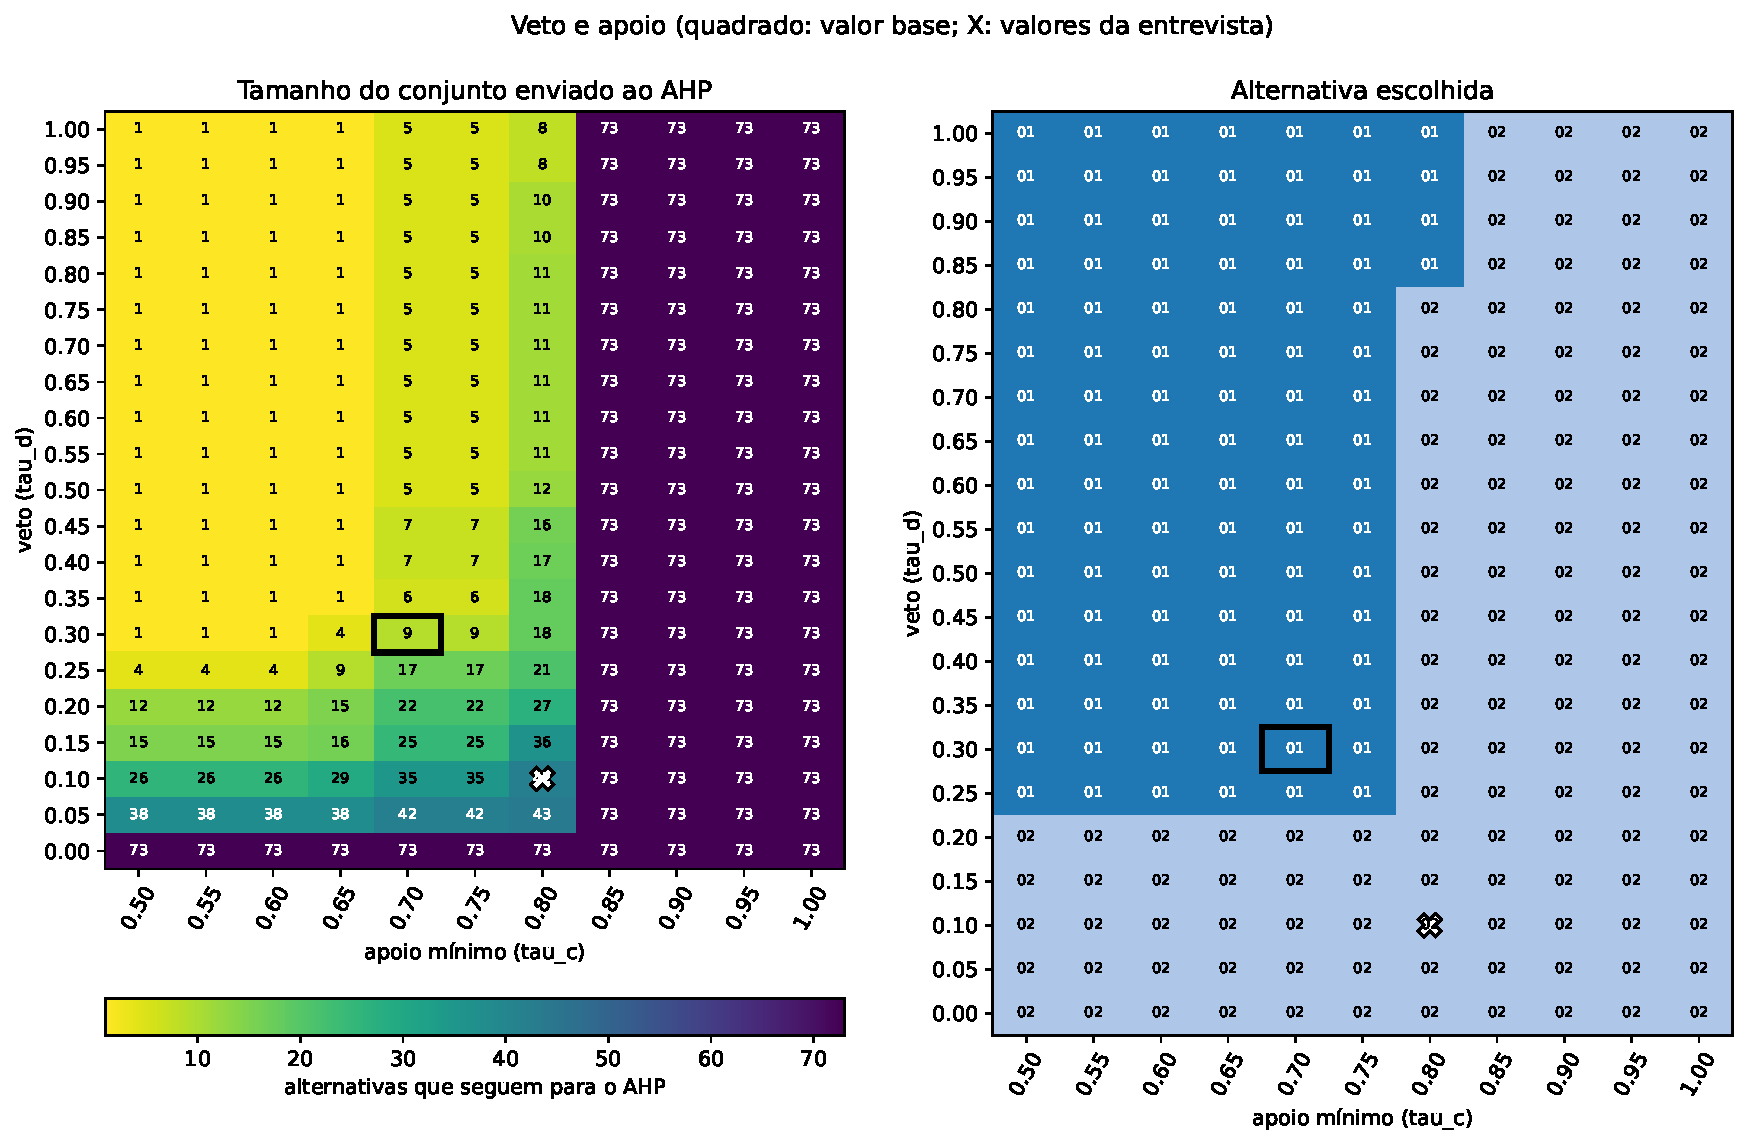
\includegraphics[width=0.92\textwidth]{mapa_calor_limiares.pdf}
\caption{Alternativas enviadas ao AHP e alternativa escolhida para cada par de apoio mínimo $\tau_c$ e veto $\tau_d$. O quadrado marca os valores adotados e o X, os declarados pelo respondente.}
\label{fig:mapa}
\end{figure*}

\begin{figure*}[!t]
\centering
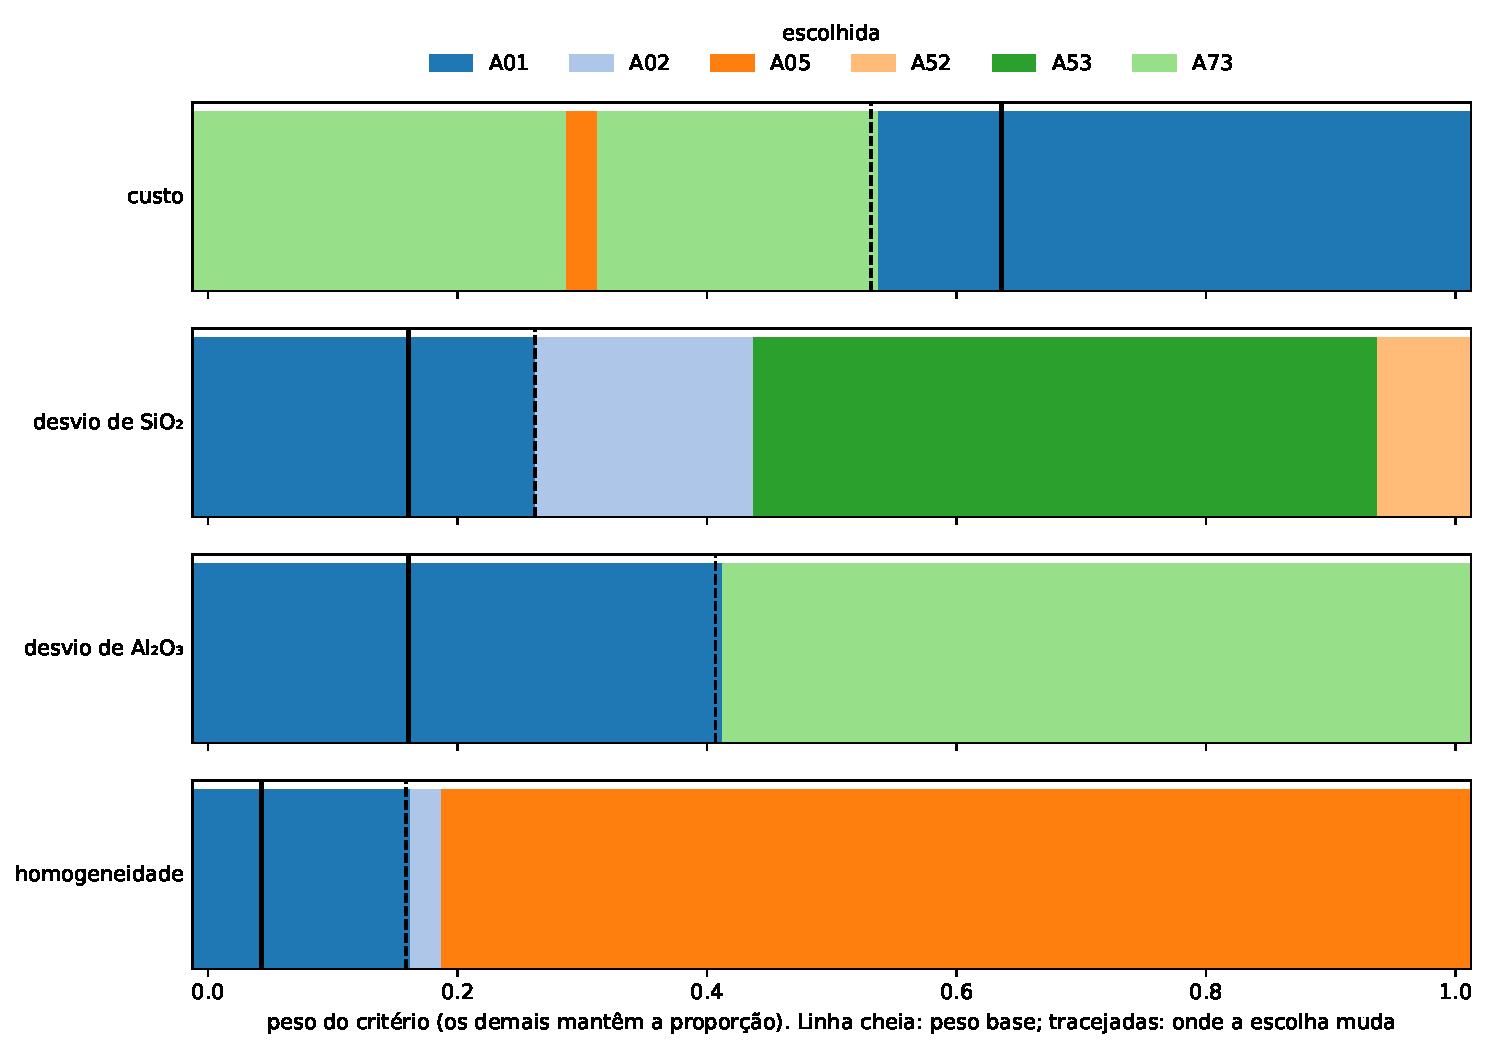
\includegraphics[width=0.85\textwidth]{sensibilidade_pesos.pdf}
\caption{Alternativa escolhida quando o peso de cada critério varia de 0 a 1, com os demais na proporção original. A linha cheia marca o peso adotado e as tracejadas, os pesos em que a escolha muda.}
\label{fig:pesos_sens}
\end{figure*}

\begin{figure*}[!t]
\centering
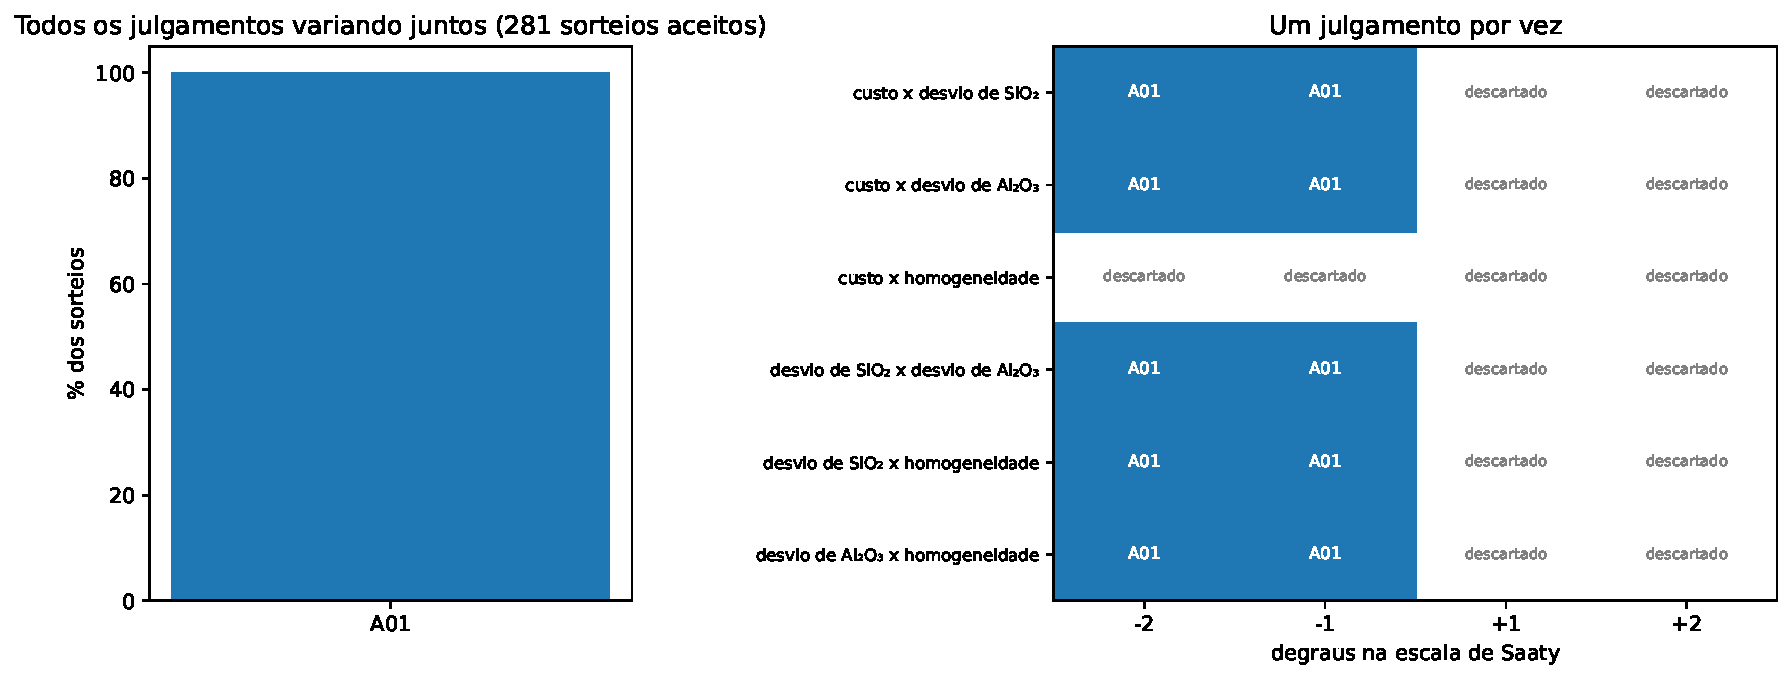
\includegraphics[width=\textwidth]{sensibilidade_julgamentos.pdf}
\caption{Alternativa escolhida quando os julgamentos do respondente variam em degraus da escala de Saaty: todos juntos, em sorteios de até um degrau, e um de cada vez, de um a dois degraus. São descartadas as variações que saem da escala ou ficam mais inconsistentes que a matriz original.}
\label{fig:julgamentos}
\end{figure*}

Em torno do caso base, variamos um grupo de parâmetros por vez, mantendo os demais nos valores base: o veto, o apoio, o número de níveis do ELECTRE~I enviados ao AHP, o modo do AHP, os pesos e os julgamentos do decisor. O número de alternativas do AHP varia por níveis inteiros, e não por cortes dentro de um nível, para evitar o desempate arbitrário. Acrescentamos o par apoio e veto em uma grade (Figura~\ref{fig:mapa}) e um caso de referência com o AHP aplicado às 73 alternativas, sem o ELECTRE~I. Os resultados estão na Tabela~\ref{tab:sens}.

\begin{table}[htbp]
\caption{Alternativa escolhida nas variações em torno do caso base}
\centering
\small
\begin{tabular}{p{0.46\columnwidth} r c}
\toprule
\textbf{Variação} & \textbf{No AHP} & \textbf{Escolhida} \\
\midrule
Caso base ($\tau_c=0{,}70$, $\tau_d=0{,}30$) & 4 & A01 \\
Veto de 0{,}25 a 0{,}50 & 9 a 1 & A01 \\
Veto de 0{,}10 a 0{,}20 & 29 a 15 & A02 \\
Apoio de 0{,}50 a 0{,}80 & 1 a 11 & A01 \\
Apoio de 0{,}85 e 0{,}90 & 17 e 73 & A02 \\
Valores declarados ($\tau_c=0{,}80$, $\tau_d=0{,}25$) & 16 & A02 \\
Dois primeiros níveis & 5 & A01 \\
Três primeiros níveis & 7 & A02 \\
AHP sobre as 73, sem ELECTRE~I & 73 & A02 \\
AHP pela razão dos valores & 4 & A73 \\
Julgamentos, 1 e 2 degraus (10 casos) & 4 a 9 & A01 \\
Julgamentos, 281 sorteios & 1 a 9 & A01 \\
\bottomrule
\end{tabular}
\label{tab:sens}
\end{table}

A A02 custa R\$~40~mil a mais que a A01, é melhor em SiO$_2$ e em homogeneidade e pior em Al$_2$O$_3$. O ELECTRE~I a deixa no segundo nível, pois a A01 a sobreclassifica ($C=0{,}78$ e $D=0{,}23$) e o inverso não vale. Quando as duas participam do AHP, ele praticamente não as separa: as prioridades são 0{,}236 e 0{,}234 com dois níveis, a favor da A01, e diferem em menos de 0{,}0001 com três níveis, quando a A73 também empata com elas. Com os valores declarados pelo respondente, 16 alternativas seguem para o AHP, e a A02 vence a A01 por 0{,}1125 a 0{,}1124. A troca de A01 por A02 nas variações da tabela, portanto, reflete a entrada da A02 no conjunto, e não uma diferença real entre as duas, que são praticamente a mesma solução. O encadeamento adotado leva à A01 pelo critério não compensatório do ELECTRE~I.

O AHP pela razão dos valores escolhe a A73, a de menor desvio de Al$_2$O$_3$ e a mais cara, e coloca a A01 na última posição entre as quatro. Isso ocorre porque a razão trata as diferenças de custo como pequenas, o que anula o peso do custo obtido na entrevista, e é a razão de usarmos a faixa de cada critério.

A escolha só muda para soluções distintas de A01 e A02 com mudanças grandes nos pesos. A A01 se mantém enquanto o peso do custo fica acima de 0{,}549 (valor adotado: 0{,}671), o da sílica abaixo de 0{,}300 (0{,}186), o da alumina abaixo de 0{,}260 (0{,}110) e o da homogeneidade abaixo de 0{,}133 (0{,}033). Fora desses valores, a escolha passa para alternativas de custo maior e melhor qualidade, como a A02, a A05 e a A73. A relação não é monótona, porque os pesos também mudam o conjunto que o ELECTRE~I envia ao AHP: no peso da alumina, a A73 vence entre 0{,}26 e 0{,}27, a A01 volta a vencer até 0{,}40, e só acima disso a A73 assume. Nas perturbações dos julgamentos da Cassotis, só valem as que não aumentam a inconsistência, já que a matriz original foi aceita com QC acima do limite: das 24 perturbações de um julgamento por vez, 10 atendem a essa condição, e dos 1000 sorteios de até um degrau em todos os julgamentos, 281. Em todas, a escolha continua sendo a A01.

\subsection{Comparação entre os Métodos e Recomendação}\label{sec:recomendacao}

Isolados, os dois métodos não respondem à mesma pergunta. O ELECTRE~I sozinho não chega a uma alternativa: ele deixa quatro alternativas incomparáveis no primeiro nível. O AHP sozinho, aplicado às 73, ordena todas e põe a A02 em primeiro e a A01 em segundo, com prioridades de 0{,}0353 e 0{,}0351. Os dois concordam que a escolha está no extremo de menor custo da fronteira e só divergem entre a A01 e a A02. A divergência vem da natureza de cada método: o AHP, compensatório, troca a desvantagem de R\$~40~mil da A02 no custo por sua vantagem em sílica e em homogeneidade, enquanto o ELECTRE~I, não compensatório, considera que a A01 supera a A02, pois ela é melhor em critérios que somam 78\% da importância e sua maior desvantagem fica dentro do veto.

Recomendamos a A01. Ela é a escolha do encadeamento definido antes dos resultados, vence com folga dentro do primeiro nível do ELECTRE~I e se mantém em todas as perturbações aceitas dos julgamentos e na maior parte das variações de veto e apoio; quando a escolha muda nessas variações, é para a A02. A A02 é uma alternativa praticamente equivalente, que pode ser preferida se a homogeneidade das receitas pesar mais na operação. Em qualquer das duas, a usina deve considerar a falta de folga em relação aos limites de qualidade antes de implementar a receita.

\section{Conclusão}\label{sec:conclusao}

A GVNS proposta encontrou soluções viáveis em todas as 15 execuções. Para os desvios de SiO$_2$ e Al$_2$O$_3$, as cinco execuções convergiram para praticamente o mesmo valor; para o custo, a amplitude dos resultados foi cerca de 0{,}9\% do menor valor observado, o que indica maior sensibilidade à semente. A comparação entre as melhores soluções de cada objetivo mostra que custo e qualidade são conflitantes: a solução de menor custo apresenta os maiores desvios, e a de menor desvio de Al$_2$O$_3$ custa cerca de 10{,}7\% a mais. Essas três soluções também definem, para cada objetivo, o menor e o maior valor usados para colocar os três objetivos na mesma escala na otimização multiobjetivo. Na comparação com a referência exata, a melhor solução de custo ficou 0{,}17\% acima do ótimo provado, a de $f_3$ coincidiu com a melhor solução obtida pelo Gurobi e a de $f_2$ ficou a $1{,}7\times10^{-5}$, em termos relativos, da melhor solução do Gurobi.

Na etapa multiobjetivo, a mesma GVNS foi aplicada à Soma Ponderada e ao $\varepsilon$-restrito, sem falhas de reparo nas 115 chamadas. O $\varepsilon$-restrito produziu 61 receitas não dominadas, distribuídas por toda a superfície de compromisso, e maior hipervolume (0{,}655 contra 0{,}584), enquanto a Soma Ponderada concentrou suas 15 receitas em cinco grupos, como esperado para um método que não alcança regiões não suportadas da fronteira. As abordagens mostraram-se complementares: a Soma Ponderada alcançou os extremos de qualidade, e o $\varepsilon$-restrito, o menor custo e o interior da fronteira. Em ambas, as cinco rodadas atingiram as mesmas regiões do espaço de objetivos, com pequena variação do hipervolume entre rodadas. As 73 receitas não dominadas da união das duas abordagens formam o conjunto de alternativas para a etapa de decisão multicritério.

Na decisão multicritério, os pesos vieram de um formulário respondido por um profissional da Cassotis: custo 0{,}671, sílica 0{,}186, alumina 0{,}110 e homogeneidade 0{,}033. O quociente de consistência dessas respostas é 0{,}20, acima do limite de 0{,}10, por causa do teto da escala de Saaty, e a devolutiva enviada não teve resposta a tempo; usamos os julgamentos como estão e registramos essa limitação. O ELECTRE~I, com apoio mínimo de 0{,}70 e veto de 0{,}30, reduziu as 73 alternativas a 4 que nenhuma outra supera, e o AHP escolheu entre elas a receita de menor custo, R\$~59{,}58 milhões, com prioridade global de 0{,}337 contra 0{,}233 da segunda colocada. É um extremo da fronteira: os desvios de SiO$_2$ e de Al$_2$O$_3$ ficam a 94\% e 95\% do caminho entre o melhor e o pior valor, e as pilhas operam a menos de 0{,}07~pp do limite superior de sílica. A escolha se mantém para o veto entre 0{,}25 e 0{,}50, para o apoio até 0{,}80 e em todas as perturbações dos julgamentos que não aumentam a inconsistência. Quando a A02, uma receita R\$~40~mil mais cara e praticamente equivalente, entra no AHP, as duas passam a disputar o primeiro lugar por diferenças mínimas de prioridade. Soluções realmente distintas, mais caras e de melhor qualidade, só aparecem se o peso do custo cair de 0{,}67 para 0{,}55 ou se o AHP usar a razão dos valores, que anula o peso do custo. As limitações são a falta de folga das pilhas em relação aos limites de qualidade, que o modelo não penaliza, a inconsistência dos julgamentos e o fato de a entrevista ter um único respondente.

\begin{table*}[!t]
\centering
{\normalsize\scshape Apêndice B: critérios das alternativas}\\[1.2ex]
\caption{Critérios das 73 alternativas avaliadas pelo ELECTRE~I: custo $f_1$ (R\$ milhões), desvios $f_2$ e $f_3$ (pp$^2$), homogeneidade $H$, nível no ELECTRE~I e prioridade global $g$ do AHP, para as que seguiram para o AHP. A escolhida pelo AHP está em negrito}
\centering
\scriptsize
\begin{tabular}{l r r r r c r @{\hspace{1.2em}} l r r r r c r}
\toprule
\textbf{Alt.} & \textbf{$f_1$} & \textbf{$f_2$} & \textbf{$f_3$} & \textbf{$H$} & \textbf{Nív.} & \textbf{$g$} & \textbf{Alt.} & \textbf{$f_1$} & \textbf{$f_2$} & \textbf{$f_3$} & \textbf{$H$} & \textbf{Nív.} & \textbf{$g$} \\
\midrule
\textbf{A01} & \textbf{59{,}58} & \textbf{6{,}75} & \textbf{6{,}44} & \textbf{0{,}860} & \textbf{1} & \textbf{0{,}173} & A38 & 62{,}82 & 2{,}81 & 4{,}01 & 0{,}941 & 12 & -- \\
A02 & 59{,}62 & 6{,}48 & 6{,}69 & 0{,}785 & 2 & -- & A39 & 62{,}96 & 2{,}81 & 4{,}07 & 0{,}975 & 13 & -- \\
A03 & 60{,}10 & 6{,}79 & 5{,}66 & 0{,}880 & 3 & -- & A40 & 62{,}98 & 4{,}48 & 2{,}76 & 0{,}871 & 14 & -- \\
A04 & 60{,}28 & 5{,}40 & 5{,}56 & 0{,}816 & 1 & 0{,}123 & A41 & 62{,}98 & 4{,}58 & 2{,}75 & 0{,}945 & 14 & -- \\
A05 & 60{,}56 & 5{,}06 & 5{,}31 & 0{,}734 & 1 & 0{,}115 & A42 & 62{,}98 & 4{,}58 & 2{,}74 & 0{,}930 & 14 & -- \\
A06 & 60{,}56 & 5{,}06 & 5{,}31 & 0{,}794 & 1 & 0{,}108 & A43 & 63{,}02 & 4{,}57 & 2{,}74 & 0{,}866 & 15 & -- \\
A07 & 60{,}84 & 4{,}72 & 5{,}06 & 0{,}981 & 1 & 0{,}092 & A44 & 63{,}14 & 2{,}47 & 4{,}03 & 0{,}816 & 13 & -- \\
A08 & 60{,}92 & 6{,}77 & 4{,}06 & 0{,}804 & 2 & -- & A45 & 63{,}14 & 2{,}47 & 4{,}01 & 0{,}823 & 13 & -- \\
A09 & 60{,}94 & 6{,}78 & 4{,}05 & 0{,}869 & 3 & -- & A46 & 63{,}14 & 2{,}81 & 3{,}80 & 0{,}856 & 13 & -- \\
A10 & 61{,}00 & 4{,}57 & 5{,}19 & 0{,}882 & 1 & 0{,}086 & A47 & 63{,}20 & 6{,}75 & 1{,}95 & 0{,}977 & 16 & -- \\
A11 & 61{,}00 & 6{,}76 & 4{,}08 & 0{,}899 & 4 & -- & A48 & 63{,}26 & 2{,}47 & 3{,}31 & 0{,}959 & 14 & -- \\
A12 & 61{,}00 & 6{,}77 & 4{,}07 & 0{,}944 & 4 & -- & A49 & 63{,}28 & 6{,}59 & 1{,}95 & 0{,}985 & 17 & -- \\
A13 & 61{,}04 & 4{,}58 & 5{,}09 & 0{,}798 & 2 & -- & A50 & 63{,}32 & 6{,}63 & 1{,}95 & 0{,}858 & 16 & -- \\
A14 & 61{,}06 & 4{,}56 & 5{,}46 & 0{,}899 & 3 & -- & A51 & 63{,}34 & 6{,}41 & 1{,}95 & 0{,}833 & 17 & -- \\
A15 & 61{,}62 & 4{,}57 & 4{,}08 & 0{,}850 & 4 & -- & A52 & 63{,}44 & 2{,}37 & 3{,}29 & 0{,}937 & 2 & -- \\
A16 & 61{,}66 & 4{,}57 & 4{,}08 & 0{,}859 & 4 & -- & A53 & 63{,}44 & 2{,}37 & 3{,}29 & 0{,}819 & 1 & 0{,}101 \\
A17 & 61{,}68 & 4{,}58 & 4{,}07 & 0{,}895 & 5 & -- & A54 & 63{,}46 & 3{,}47 & 2{,}75 & 0{,}896 & 16 & -- \\
A18 & 61{,}68 & 4{,}59 & 4{,}06 & 0{,}928 & 5 & -- & A55 & 63{,}46 & 3{,}47 & 2{,}74 & 0{,}906 & 16 & -- \\
A19 & 61{,}94 & 7{,}00 & 2{,}85 & 0{,}796 & 5 & -- & A56 & 63{,}48 & 3{,}47 & 2{,}75 & 0{,}965 & 17 & -- \\
A20 & 62{,}04 & 3{,}47 & 4{,}93 & 0{,}896 & 6 & -- & A57 & 63{,}58 & 3{,}47 & 2{,}76 & 0{,}929 & 18 & -- \\
A21 & 62{,}06 & 3{,}47 & 4{,}75 & 0{,}873 & 7 & -- & A58 & 63{,}80 & 2{,}81 & 2{,}75 & 0{,}848 & 17 & -- \\
A22 & 62{,}08 & 3{,}47 & 4{,}54 & 0{,}883 & 7 & -- & A59 & 63{,}86 & 2{,}80 & 2{,}75 & 0{,}868 & 18 & -- \\
A23 & 62{,}10 & 6{,}99 & 2{,}70 & 0{,}973 & 6 & -- & A60 & 63{,}86 & 2{,}81 & 2{,}75 & 1{,}057 & 19 & -- \\
A24 & 62{,}18 & 6{,}70 & 2{,}75 & 0{,}785 & 5 & -- & A61 & 63{,}98 & 4{,}57 & 1{,}95 & 0{,}948 & 19 & -- \\
A25 & 62{,}20 & 3{,}48 & 4{,}09 & 0{,}865 & 8 & -- & A62 & 64{,}02 & 4{,}58 & 1{,}95 & 0{,}935 & 20 & -- \\
A26 & 62{,}20 & 6{,}76 & 2{,}75 & 0{,}860 & 9 & -- & A63 & 64{,}02 & 4{,}58 & 1{,}92 & 0{,}925 & 20 & -- \\
A27 & 62{,}22 & 3{,}48 & 4{,}09 & 0{,}753 & 5 & -- & A64 & 64{,}08 & 4{,}58 & 1{,}95 & 0{,}882 & 21 & -- \\
A28 & 62{,}22 & 6{,}72 & 2{,}75 & 0{,}963 & 10 & -- & A65 & 64{,}54 & 3{,}43 & 1{,}95 & 0{,}931 & 22 & -- \\
A29 & 62{,}24 & 3{,}47 & 4{,}08 & 0{,}860 & 8 & -- & A66 & 64{,}54 & 3{,}47 & 1{,}95 & 0{,}935 & 22 & -- \\
A30 & 62{,}24 & 6{,}94 & 2{,}60 & 0{,}864 & 10 & -- & A67 & 64{,}58 & 3{,}47 & 1{,}94 & 0{,}917 & 23 & -- \\
A31 & 62{,}26 & 3{,}46 & 4{,}08 & 0{,}919 & 9 & -- & A68 & 64{,}60 & 3{,}42 & 1{,}94 & 0{,}900 & 24 & -- \\
A32 & 62{,}28 & 3{,}48 & 4{,}06 & 0{,}917 & 10 & -- & A69 & 65{,}06 & 2{,}81 & 1{,}95 & 0{,}931 & 25 & -- \\
A33 & 62{,}32 & 7{,}00 & 2{,}53 & 0{,}922 & 11 & -- & A70 & 65{,}22 & 2{,}81 & 1{,}95 & 0{,}952 & 26 & -- \\
A34 & 62{,}40 & 7{,}05 & 2{,}45 & 0{,}815 & 11 & -- & A71 & 65{,}22 & 2{,}81 & 1{,}95 & 0{,}909 & 26 & -- \\
A35 & 62{,}80 & 2{,}81 & 4{,}39 & 0{,}944 & 11 & -- & A72 & 65{,}24 & 2{,}82 & 1{,}94 & 0{,}898 & 27 & -- \\
A36 & 62{,}80 & 2{,}81 & 4{,}27 & 0{,}926 & 11 & -- & A73 & 65{,}46 & 2{,}68 & 1{,}69 & 0{,}786 & 1 & 0{,}119 \\
A37 & 62{,}82 & 2{,}81 & 4{,}06 & 0{,}830 & 1 & 0{,}084 &  &  &  &  &  &  &  \\
\bottomrule
\end{tabular}

\label{tab:apendice}
\end{table*}

\section*{Apêndice A: formulário da entrevista}

\begingroup\footnotesize

\textbf{Seção 1, apresentação.} Uma usina siderúrgica precisa decidir como compor 10 pilhas de minério que alimentam dois equipamentos de sinterização. Existem 73 composições candidatas, todas eficientes: nenhuma é melhor que outra em todos os aspectos ao mesmo tempo. Escolher entre elas depende do que mais importa para a usina. Pedimos que você responda como a pessoa responsável por essa escolha. São quatro aspectos: custo é o gasto com a compra dos minérios; sílica e alumina medem o quanto o teor de cada pilha fica longe do alvo do equipamento; receita parecida mede o quanto as pilhas de um mesmo equipamento seguem receitas (proporções de minérios) semelhantes, o que simplifica o trabalho no pátio. Para cada aspecto, damos o pior e o melhor valor existentes entre as 73 composições.

\textbf{Seção 2, o que mais importa.} Em cada pergunta, considere a melhoria do pior para o melhor valor existente entre as composições, em um aspecto de cada vez. Duas perguntas de resposta única, obrigatórias: ``Se você pudesse melhorar só um aspecto, do pior para o melhor valor, qual traria mais valor para a usina?'' e ``Qual dos quatro traria menos valor, ou seja, qual você abriria mão primeiro?''. As opções, iguais nas duas perguntas, são:
\begin{itemize}\setlength{\itemsep}{0pt}
\item Custo: a compra de minério cai de R\$~65,5 milhões para R\$~59,6 milhões (economia de R\$~5,9 milhões, cerca de 10\%).
\item Sílica: o desvio típico do teor de sílica de cada pilha em relação ao alvo do equipamento cai de 0,84 para 0,49 ponto percentual.
\item Alumina: o desvio típico do teor de alumina de cada pilha em relação ao alvo do equipamento cai de 0,82 para 0,41 ponto percentual.
\item Receita parecida: a receita de cada pilha difere da receita comum do equipamento em 37\% dos caminhões, em vez de 53\%.
\end{itemize}

\textbf{Seção 3, quanto mais importa.} Para cada par, diga quanto uma melhoria vale mais que a outra, sempre do pior para o melhor valor do aspecto. Seis perguntas de resposta única, obrigatórias, uma para cada par, na ordem custo e sílica, custo e alumina, custo e receita parecida, sílica e alumina, sílica e receita parecida, alumina e receita parecida. Modelo da pergunta, para o par $X$ e $Y$: ``Quanto vale mais melhorar $X$ ou melhorar $Y$?''. Opções, em que \textit{nível} percorre ``extremamente'' (9), ``muito fortemente'' (7), ``fortemente'' (5) e ``moderadamente'' (3):
\begin{itemize}\setlength{\itemsep}{0pt}
\item Melhorar $X$ vale \textit{nível} mais que melhorar $Y$ (valor positivo, de 9 a 3);
\item As duas melhorias valem o mesmo (1);
\item Melhorar $Y$ vale \textit{nível} mais que melhorar $X$ (valor negativo, de $-3$ a $-9$).
\end{itemize}

\textbf{Seção 4, como comparar duas composições.} Ao comparar duas composições, uma pode ser melhor em alguns aspectos e pior em outros. As duas perguntas seguintes definem quando você aceita dizer que uma composição supera a outra.

Primeira pergunta: ``Você aceita uma composição que seja pior em um aspecto desde que compense nos outros. Qual a maior piora que você toleraria em qualquer aspecto isolado?'' Texto de apoio: ``Meça como fração da faixa entre o melhor e o pior valor. Exemplo de 25\% da faixa: R\$~1,5 milhão a mais de custo, ou sílica e alumina cerca de 0,09 ponto percentual mais longe do alvo.'' Opções: até 10\%, 25\%, 40\% ou 50\% da faixa, cada uma com uma frase que a explica.

Segunda pergunta: ``Para considerar que a composição A é `pelo menos tão boa quanto' a B e descartar a B, os aspectos em que A é melhor ou igual a B precisam somar quanto da importância total?'' Texto de apoio: ``Por exemplo, se custo e sílica somam 70\% da importância e A é melhor ou igual a B nesses dois, então 70\% da importância está a favor de A.'' Opções: pelo menos 60\%, 70\%, 80\% ou 90\%, cada uma com uma frase que a explica.

\textbf{Seção 5, para terminar.} Uma pergunta de texto livre, opcional: ``Há algum aspecto importante para a usina que ficou de fora, ou alguma observação sobre as suas respostas?''

\endgroup

\begin{thebibliography}{99}

\bibitem{aula02}
L.~B.~Real, ``Da construção de soluções às metaheurísticas: representação, busca local e VNS,'' notas de aula (Aula~02), Teoria da Decisão, Universidade Federal de Minas Gerais, Belo Horizonte, 2026.

\bibitem{aula04}
L.~B.~Real, ``Penalidades e otimização vetorial,'' notas de aula (Aula~04), Teoria da Decisão, Universidade Federal de Minas Gerais, Belo Horizonte, 2026.

\bibitem{case_cassotis}
Cassotis Consulting, ``Otimização de custo e qualidade na formação de pilhas de minério,'' case da disciplina Teoria da Decisão, Engenharia de Sistemas, Universidade Federal de Minas Gerais, Belo Horizonte, 2026/2.

\bibitem{blank_deb2020}
J.~Blank e K.~Deb, ``Pymoo: Multi-Objective Optimization in Python,''
\textit{IEEE Access}, vol.~8, 2020. doi: 10.1109/ACCESS.2020.2990567.

\bibitem{friedman1937}
M.~Friedman, ``The use of ranks to avoid the assumption of normality implicit
in the analysis of variance,'' \textit{Journal of the American Statistical
Association}, vol.~32, n.~200, pp.~675--701, 1937.
doi: 10.1080/01621459.1937.10503522.

\bibitem{wilcoxon1945}
F.~Wilcoxon, ``Individual comparisons by ranking methods,''
\textit{Biometrics Bulletin}, vol.~1, n.~6, pp.~80--83, 1945.
doi: 10.2307/3001968.

\bibitem{derrac2011}
J.~Derrac, S.~García, D.~Molina e F.~Herrera, ``A practical tutorial on the use
of nonparametric statistical tests as a methodology for comparing evolutionary
and swarm intelligence algorithms,'' \textit{Swarm and Evolutionary
Computation}, vol.~1, n.~1, pp.~3--18, 2011. doi: 10.1016/j.swevo.2011.02.002.

\bibitem{scipy2020}
P.~Virtanen \textit{et al.}, ``SciPy 1.0: fundamental algorithms for scientific
computing in Python,'' \textit{Nature Methods}, vol.~17, n.~3, pp.~261--272,
2020. doi: 10.1038/s41592-019-0686-2.

\bibitem{zitzler1999}
E.~Zitzler e L.~Thiele, ``Multiobjective evolutionary algorithms: a comparative
case study and the strength Pareto approach,'' \textit{IEEE Transactions on
Evolutionary Computation}, vol.~3, n.~4, pp.~257--271, 1999.

\bibitem{gams_eps}
GAMS Development Corporation, ``epscm.gms: eps-Constraint Method for
Multiobjective Optimization,'' \textit{GAMS Model Library},
\url{https://www.gams.com/latest/gamslib_ml/libhtml/gamslib_epscm.html}.
Acesso em 13 out. 2026.

\bibitem{aula10}
L.~B.~Real, ``Síntese de critérios: teoria multiatributo e AHP,'' notas de aula (Aula~10), Teoria da Decisão, Universidade Federal de Minas Gerais, Belo Horizonte, 2026.

\bibitem{aula_electre}
L.~B.~Real, ``Métodos de sobreclassificação: ELECTRE~I,'' videoaula, Teoria da Decisão, Universidade Federal de Minas Gerais, Belo Horizonte, 2026.

\bibitem{figueira2005}
J.~Figueira, V.~Mousseau e B.~Roy, ``ELECTRE methods,'' em \textit{Multiple Criteria Decision Analysis: State of the Art Surveys}, J.~Figueira, S.~Greco e M.~Ehrgott, Eds. Springer, 2005, cap.~4. doi: 10.1007/0-387-23081-5\_4.

\bibitem{saaty1994}
T.~L.~Saaty, ``How to make a decision: the analytic hierarchy process,'' \textit{Interfaces}, vol.~24, n.~6, pp.~19--43, 1994. doi: 10.1287/inte.24.6.19.

\end{thebibliography}

\end{document}
